% DeSTiL paper, Vietnamese, IEEE conference format. Version 2 (2026-11-04), after the internal review.
% Compile: XeLaTeX (recommended) or pdfLaTeX, then BibTeX, then twice more.
%   latexmk -xelatex pp3_paper_vi.tex
% Overleaf: upload this folder together with ../figures (or put the PNGs in
% ./figures) and set the compiler to XeLaTeX.
% \tbd marks numbers that come from runs still to be done (none left).
\documentclass[conference]{IEEEtran}

\usepackage{iftex}
\ifXeTeX
  \usepackage{fontspec}
  \setmainfont{TeX Gyre Termes}
  \usepackage{polyglossia}
  \setdefaultlanguage{vietnamese}
\else\ifLuaTeX
  \usepackage{fontspec}
  \setmainfont{TeX Gyre Termes}
  \usepackage[vietnamese]{babel}
\else
  \usepackage[T5]{fontenc}
  \usepackage[utf8]{inputenc}
  \usepackage[vietnamese]{babel}
\fi\fi

\usepackage{amsmath,amssymb}
\usepackage{graphicx}
\usepackage{booktabs}
\usepackage{multirow}
\usepackage{array}
\usepackage{xcolor}
\usepackage{cite}
\usepackage[colorlinks=true,linkcolor=blue!60!black,citecolor=blue!60!black,urlcolor=blue!60!black]{hyperref}
\graphicspath{{figures/}{../figures/}}
\usepackage{placeins}            % FloatBarrier before the appendix and references
\usepackage{flafter}             % a float never appears before the text position that defines it
\raggedbottom                    % no stretched gaps when a float moves to the next column
\makeatletter                    % float-only pages start at the top, not centred
\setlength{\@fptop}{0pt}\setlength{\@dblfptop}{0pt}
\makeatother
% Let LaTeX put more and larger floats on a page, so wide figures do not pile up at the end.
\renewcommand{\topfraction}{0.9}
\renewcommand{\dbltopfraction}{0.9}
\renewcommand{\bottomfraction}{0.8}
\renewcommand{\textfraction}{0.07}
\renewcommand{\floatpagefraction}{0.8}
\renewcommand{\dblfloatpagefraction}{0.8}
\setcounter{topnumber}{4}
\setcounter{dbltopnumber}{4}
\setcounter{totalnumber}{6}

\newcommand{\mi}{\ensuremath{-}}            % minus sign in text and tables
\newcommand{\pl}{\ensuremath{+}}
\newcommand{\qhat}{\ensuremath{\hat{q}}}
\newcommand{\best}[1]{\textbf{#1}}
\newcommand{\ok}{\ensuremath{\checkmark}}
\newcommand{\nok}{\ensuremath{\times}}
\newcommand{\tbd}{\textcolor{red}{[chờ]}}
\newcommand{\Hmlp}{H\textsubscript{MLP}}
\newcommand{\Hattn}{H\textsubscript{Attn}}
\newcommand{\Htg}{H\textsubscript{TG}}

\begin{document}

\title{Question-Aware Visual Token Selection with an Attention-Distilled Scorer for DeepStack Vision-Language Models}

\author{
\IEEEauthorblockN{Nguyễn Thiện Thanh, Nguyễn Trung Hiếu, Gia Bảo}
\IEEEauthorblockA{Giảng viên hướng dẫn: Lê Phú Nguyên}
}

\maketitle

\begin{abstract}
Mô hình thị giác--ngôn ngữ (VLM) dành phần lớn chuỗi đầu vào cho token ảnh, trong khi một câu hỏi thường chỉ cần một phần nhỏ của ảnh. Các phương pháp chọn token có điều kiện theo câu hỏi trước LLM, như CDPruner, dùng một điểm liên quan thủ công (độ tương đồng cosine giữa token ảnh và câu lệnh) làm trọng số chất lượng của một quá trình điểm xác định (DPP). Bài báo này đề xuất \textbf{DeSTiL} (\emph{DeepStack Token selection via attention distiLlation}), thay điểm thủ công đó bằng một \emph{score head} nhỏ (2 triệu tham số) được huấn luyện để dự đoán attention văn bản$\rightarrow$ảnh của chính LLM full-token, và xử lý cả ba luồng đặc trưng DeepStack của Qwen3-VL. Trên Qwen3-VL-2B, ở cùng số token, DeSTiL tốt hơn chọn ngẫu nhiên, DivPrune, FastV-style và CDPruner ở mọi mức budget trên GQA, MMBench và MME perception; so với CDPruner, DeSTiL hơn \pl7,2 điểm trên GQA ở 5,7\% token và \pl2,7 điểm ở 22\%. Giữ 22\% token ảnh, DeSTiL đạt non-inferiority so với mô hình full trên GQA testdev (\mi0,50 điểm; cận dưới một phía \mi0,88, biên 1 điểm). Với 5,7\% token, DeSTiL mất 4,0 điểm trên GQA, so với 11,2 của DivPrune. Trên POPE, DeSTiL không làm tăng ảo giác vật thể: từ 11\% token, accuracy và F1 không khác mô hình full (non-inferiority, bootstrap theo ảnh); ở 5,7\% token, DeSTiL chỉ mất 1,1 điểm, so với 9,0 của DivPrune và 10,6 của CDPruner, vì các baseline bỏ sót vật thể được hỏi. Trên ảnh độ phân giải cao của MME, DeSTiL giảm FLOPs prefill của LLM 5,2 lần ở 22\% token, và giảm thời gian chọn token + prefill 1,5 lần ở batch 1. Điểm yếu chính là các tác vụ phải đọc chữ: điểm MME cognition giảm từ 533,6 xuống 397,1 ở mức 22\%, và mọi phương pháp chọn token đều giảm tương tự. Trên Qwen3-VL-4B, với cùng phương pháp và siêu tham số, DeSTiL vẫn tốt nhất trên GQA, MMBench, POPE và MME perception từ 5,7\% đến 22,4\% token và có điểm cao nhất trên GQA, POPE và MME perception ở 33,4\%, và giảm thời gian chọn token + prefill trên MME 2,5 lần ở 22\% token. Bài báo cũng phân tích attention sink trong nhãn teacher và đề xuất một biến thể dễ diễn giải cho vùng focus theo câu hỏi.
\end{abstract}

\begin{IEEEkeywords}
mô hình thị giác--ngôn ngữ, cắt tỉa token ảnh, chưng cất attention, quá trình điểm xác định, Qwen3-VL, DeepStack
\end{IEEEkeywords}

% ======================================================================
\section{Giới thiệu}
\label{sec:intro}

Một VLM như Qwen3-VL~\cite{qwen2025qwen3vl} biến ảnh thành một dãy token rồi ghép với câu hỏi để LLM xử lý. Số token ảnh tăng theo độ phân giải. Với Qwen3-VL-2B, mỗi token ứng với một ô $32\times32$ pixel; ảnh GQA cho 64--1200 token, còn ảnh MME có thể lên tới 16\,320 token. Chi phí của LLM (tính toán ở bước prefill, bộ nhớ KV cache) tăng theo độ dài chuỗi, trong khi phần lớn câu hỏi chỉ liên quan tới một vài vùng nhỏ của ảnh.

Các phương pháp giảm token ảnh hiện có đi theo ba hướng. Hướng thứ nhất cắt token bên trong LLM theo attention (FastV~\cite{chen2024fastv}, SparseVLM~\cite{zhang2025sparsevlm}, PyramidDrop~\cite{xing2025pyramiddrop}); cách này cần trọng số attention tường minh nên không dùng được FlashAttention~\cite{dao2024flashattention2}, và vẫn chạy các lớp đầu với đủ token. Hướng thứ hai cắt token trước LLM mà không phụ thuộc câu hỏi (ToMe~\cite{bolya2023tome}, VisionZip~\cite{yang2025visionzip}, DivPrune~\cite{alvar2025divprune}), nên mọi câu hỏi trên cùng một ảnh nhận cùng một tập token. Hướng thứ ba cắt token trước LLM có điều kiện theo câu hỏi; gần nhất với bài báo này là CDPruner~\cite{zhang2025cdpruner}, phương pháp nhân ma trận tương đồng giữa các token ảnh với điểm liên quan tới câu lệnh rồi chọn tập con bằng DPP, trong đó điểm liên quan là độ tương đồng cosine thủ công, không học.

Điểm liên quan cosine chỉ đo token ảnh ``giống'' câu lệnh tới đâu trong không gian embedding, không đo LLM \emph{thực sự dùng} token nào để trả lời. Tín hiệu thứ hai có sẵn trong attention văn bản$\rightarrow$ảnh của LLM, nhưng đọc nó lúc suy luận vừa đắt vừa quá muộn. DeSTiL học trước một mạng nhỏ để \emph{dự đoán} bản đồ attention đó từ token ảnh và câu hỏi, rồi dùng dự đoán làm trọng số chất lượng cho DPP, trước khi LLM chạy.

Qwen3-VL còn có DeepStack~\cite{meng2024deepstack}: ba mức đặc trưng trung gian của ViT được cộng vào hidden state ở lớp 0--2 của LLM tại vị trí token ảnh. Một bộ chọn token cho mô hình này phải giữ bốn luồng (luồng chính và ba mức DeepStack) nhất quán với nhau. Theo khảo sát của các tác giả, chưa có phương pháp cắt token nào đã công bố bàn tới trường hợp này; bài báo mô tả một cách xử lý đơn giản (Mục~\ref{sec:fold}).

Đóng góp chính của bài báo là một trọng số chất lượng học được cho DPP có điều kiện, chưng cất từ attention văn bản$\rightarrow$ảnh của chính LLM. Trên tập phát triển, cùng một DPP với điểm thủ công (DSFold-D, cùng họ với CDPruner) mất 11,05 điểm ở budget 5,7\%, còn với score head học được chỉ mất 4,35 điểm (\pl6,70; $p<10^{-10}$); trên tập test, DeSTiL hơn CDPruner \pl1,82 đến \pl7,23 điểm trên GQA testdev. Bài báo cũng đưa ra một cách chọn token cho kiến trúc DeepStack, giữ bốn luồng nhất quán kèm bước gộp (fold) đặc trưng DeepStack của token bị bỏ; phân tích attention sink trong nhãn teacher cùng các chỉ số vùng có định nghĩa hình thức và một nhãn tương phản cho biến thể dễ diễn giải DeSTiL-fc; và một quy trình đánh giá ghép cặp với non-inferiority trên năm benchmark không gộp chung (GQA, MMBench, MME, POPE, ScienceQA-IMG), với tập phát triển, tập xác nhận và tập test tách biệt. Cuối cùng, phương pháp được kiểm chứng trên mô hình thứ hai, Qwen3-VL-4B, với cùng siêu tham số.

% ======================================================================
\section{Công trình liên quan}
\label{sec:related}

\textbf{VLM và token ảnh.} Các VLM hiện nay nối một bộ mã hóa ảnh ViT~\cite{dosovitskiy2021vit} với một LLM, qua Q-Former như BLIP-2~\cite{li2023blip2} hoặc qua một lớp chiếu đơn giản như LLaVA~\cite{liu2023llava,liu2024llava15}. Các thế hệ sau tăng độ phân giải và do đó tăng số token: InternVL~\cite{chen2024internvl} và LLaVA-OneVision~\cite{li2024llavaonevision} chia ảnh thành nhiều ô, còn Qwen2-VL~\cite{wang2024qwen2vl}, Qwen2.5-VL~\cite{bai2025qwen25vl} và Qwen3-VL~\cite{qwen2025qwen3vl} xử lý ảnh ở độ phân giải gốc với M-RoPE, nên số token ảnh thay đổi theo kích thước ảnh. Qwen3-VL dùng bộ mã hóa họ SigLIP~2~\cite{tschannen2025siglip2} và DeepStack~\cite{meng2024deepstack}. Khảo sát của Jin và cộng sự~\cite{jin2025survey} tổng hợp các hướng làm VLM hiệu quả; bài báo này tập trung vào giảm token ảnh lúc suy luận mà không huấn luyện lại VLM.

\textbf{Nén token có huấn luyện VLM.} Một nhóm phương pháp thay đổi kiến trúc hoặc huấn luyện lại VLM để dùng ít token. TokenPacker~\cite{li2024tokenpacker} thiết kế lại bộ chiếu theo hướng thô--tinh; Matryoshka Multimodal Models~\cite{cai2024matryoshka} học biểu diễn lồng nhau ở nhiều mức số token; LLaVA-Mini~\cite{zhang2025llavamini} trộn thông tin ảnh vào token văn bản trước LLM rồi nén ảnh xuống một token; ATP-LLaVA~\cite{ye2024atpllava} và Dynamic-LLaVA~\cite{huang2025dynamicllava} học các mô-đun quyết định token nào được giữ bên trong LLM. Ở ViT, DynamicViT~\cite{rao2021dynamicvit} học một bộ dự đoán token cần giữ cùng với mạng chính. Các phương pháp này fine-tune toàn bộ hoặc một phần mô hình; DeSTiL giữ nguyên VLM và chỉ học một score head 2 triệu tham số bên ngoài.

\textbf{Cắt token bên trong LLM.} FastV~\cite{chen2024fastv} nhận thấy attention tới token ảnh giảm mạnh sau lớp 2 và cắt các token nhận attention thấp từ lớp đó. SparseVLM~\cite{zhang2025sparsevlm} dùng các token văn bản liên quan để chấm điểm token ảnh bên trong LLM. PyramidDrop~\cite{xing2025pyramiddrop} cắt dần theo từng giai đoạn. FitPrune~\cite{ye2024fitprune} chọn tỉ lệ cắt cho từng lớp bằng cách khớp phân phối attention trước và sau khi cắt; VTW~\cite{lin2024vtw} rút toàn bộ token ảnh sau một lớp nhất định; TopV~\cite{yang2025topv} chọn token bằng một bài toán tối ưu lúc suy luận, tương thích với các kernel attention nhanh; FlowCut~\cite{tong2025flowcut} chấm điểm token theo dòng thông tin giữa các lớp. Các nghiên cứu phân tích gần đây chỉ ra rằng tiêu chí attention ở lớp nông thiên về vị trí của token trong ảnh~\cite{endo2025feather}, và chọn theo độ trùng lặp có thể ngang hoặc tốt hơn chọn theo attention~\cite{wen2025dart,wen2025rightproblem}. Kết quả của FastV-style trên GQA, MMBench và POPE (Mục~\ref{sec:results}) nhất quán với các nhận xét này. Mọi phương pháp trong nhóm cần trọng số attention tường minh hoặc chạy các lớp đầu của LLM với đủ token.

\textbf{Cắt và gộp token trước LLM.} ToMe~\cite{bolya2023tome} gộp các token giống nhau. LLaVA-PruMerge~\cite{shang2024prumerge} và VisionZip~\cite{yang2025visionzip} chọn token theo attention của token [CLS] trong bộ mã hóa ảnh; VisPruner~\cite{zhang2024vispruner} kết hợp attention của [CLS] với một tập token đa dạng; HiRED~\cite{arif2025hired} dùng attention của [CLS] để phân bổ budget giữa các ô của ảnh độ phân giải cao, còn GlobalCom$^2$~\cite{liu2026globalcom2} dùng ảnh thu nhỏ toàn cục để điều khiển mức nén của từng ô. Qwen3-VL không có token [CLS], nên các phương pháp này không áp dụng trực tiếp. MADTP~\cite{cao2024madtp} cắt token theo mức căn chỉnh giữa hai phương thức, và TRIM~\cite{song2025trim} chọn token theo độ tương đồng CLIP giữa token ảnh và câu hỏi. iLLaVA~\cite{hu2026illava} gộp token cả trong bộ mã hóa ảnh và trong LLM, và VScan~\cite{zhang2025vscan} kết hợp quét toàn cục--cục bộ trong bộ mã hóa với cắt ở lớp giữa của LLM. DivPrune~\cite{alvar2025divprune} chọn tập đa dạng nhất theo tiêu chí max--min, không phụ thuộc câu hỏi. Với video, DyCoke~\cite{tao2024dycoke}, PruneVid~\cite{huang2024prunevid}, FrameFusion~\cite{fu2025framefusion} và HoliTom~\cite{shao2025holitom} khai thác thêm sự trùng lặp giữa các khung hình; bài báo này xét ảnh tĩnh.

\textbf{DPP có điều kiện.} DPP~\cite{kulesza2012dpp} cân bằng chất lượng và đa dạng của một tập con; MAP tham lam~\cite{chen2018fastmap} giải xấp xỉ trong $O(NK^2)$. CDPruner~\cite{zhang2025cdpruner} dùng kernel $\mathrm{diag}(\tilde r)\,S\,\mathrm{diag}(\tilde r)$, với $\tilde r$ là cosine giữa token ảnh và embedding trung bình của câu lệnh, chuẩn hóa min--max; phương pháp không cần huấn luyện. DeSTiL dùng cùng dạng kernel, nhưng thay $\tilde r$ bằng $\qhat$ do score head dự đoán. Phần so sánh với CDPruner vì vậy cho biết lợi ích đến từ trọng số học được hay chỉ từ DPP có điều kiện.

\textbf{Chưng cất và attention sink.} Chưng cất tri thức~\cite{hinton2015distilling} huấn luyện một mô hình nhỏ bắt chước phân phối đầu ra của một mô hình lớn; DeSTiL áp dụng ý tưởng này cho bản đồ attention văn bản$\rightarrow$ảnh, với LLM đóng băng làm teacher và score head làm student. Transformer dồn attention vào một số token ít mang thông tin~\cite{xiao2024sinks}, ViT sinh ra các token ``register'' có chuẩn lớn ở nền ảnh~\cite{darcet2024registers}, và trong VLM, LLM dành attention lớn cho các token ảnh không liên quan tới câu hỏi~\cite{kang2025sink}. Bài báo quan sát thấy hiện tượng tương tự trong nhãn teacher (Mục~\ref{sec:fc}).

\textbf{Benchmark.} GQA~\cite{hudson2019gqa}, MMBench~\cite{liu2024mmbench}, MME~\cite{fu2023mme}, POPE~\cite{li2023pope} (ảo giác vật thể) và ScienceQA-IMG~\cite{lu2022scienceqa}.

% ======================================================================
\section{Phương pháp}
\label{sec:method}

\begin{figure*}[!t]
\centering
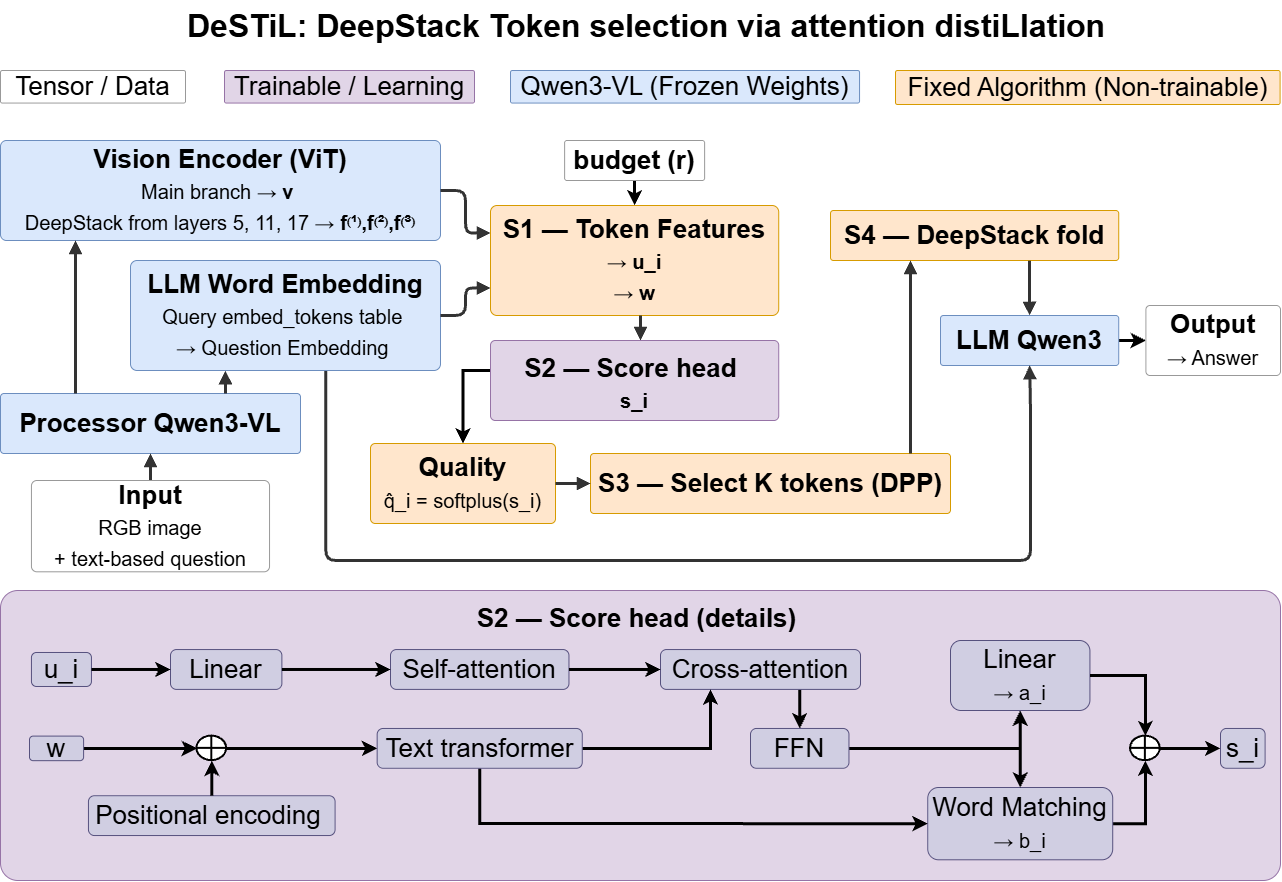
\includegraphics[width=\textwidth]{DeSTiL_architecture.png}
\caption{Luồng suy luận của DeSTiL. Xanh: Qwen3-VL, đóng băng; tím: score head \Htg, thành phần duy nhất được huấn luyện; cam: thuật toán cố định. S1 tạo đặc trưng $u_i$ cho mỗi token ảnh và $w$ cho câu hỏi; S2 dự đoán điểm $s_i=a_i+b_i$ (chi tiết ở khung dưới); S3 chọn $K$ token bằng DPP với chất lượng $\qhat_i=\mathrm{softplus}(s_i)$; S4 gộp đặc trưng DeepStack của token bị bỏ vào token giữ lại trước khi đưa vào LLM.}
\label{fig:arch}
\end{figure*}

\subsection{Bài toán và ký hiệu}
\label{sec:setting}
Sau ViT và PatchMerger, ảnh cho ra $N$ token $v_i\in\mathbb{R}^{2048}$ trên lưới $H'\times W'$, và ba mức đặc trưng DeepStack $f_i^{(l)}$, $l=1..3$ (lấy từ ViT lớp 5, 11, 17). Budget được cho bởi \emph{tỉ lệ giữ token mục tiêu} $r\in(0,1]$: tỉ lệ số token ảnh muốn giữ lại trên tổng số $N$ token ảnh của một ảnh, được chọn trước cho mỗi mức budget. Với mỗi ảnh, bộ chọn giữ $K=\lceil rN\rceil$ token (số token giữ lại, làm tròn lên) và bỏ $N-K$ token còn lại. LLM nhận các $v$ giữ lại \emph{tại đúng vị trí M-RoPE gốc} $(t,h,w)$, và đặc trưng DeepStack của chúng. Toàn bộ Qwen3-VL đóng băng; chỉ score head được huấn luyện. Bộ chọn gồm bốn bước (step), ký hiệu S1--S4 trên Hình~\ref{fig:arch} và trong các mục dưới đây: đặc trưng token (S1), score head (S2), chọn token bằng DPP (S3) và fold DeepStack (S4).

Bài báo dùng năm mức budget $r\in\{1/18,\,1/9,\,2/9,\,1/3,\,1/2\}$, ký hiệu L1--L5. Mọi phương pháp được so sánh ở bốn mức L1--L4 (từ 5,6\% đến 33,3\% token), trên cả hai mô hình và năm benchmark. Mức L5 (50\%) chỉ được dùng cho biến thể DeSTiL-fc (Mục~\ref{sec:fc}): biến thể này dành $\rho=25\%$ của $K$ cho vùng focus, nên được đánh giá ở budget lớn hơn để phần context còn đủ token. Ở L5, DeSTiL-fc được chạy trên tập test GQA, MMBench và MME của Qwen3-VL-2B (Bảng~\ref{tab:ni}), còn DeSTiL được chạy trên tập phát triển tune2k để phân tích hình dạng vùng (Mục~\ref{sec:region}); các baseline không được chạy ở L5. Vì $K$ được làm tròn lên, số token thật sự giữ lại không ít hơn $rN$ và thường nhiều hơn một chút, nhất là với ảnh ít token. Vì vậy bài báo báo cáo \emph{tỉ lệ giữ token thực tế} của mỗi tập dữ liệu, bằng tổng $K$ chia cho tổng $N$ trên mọi ảnh của tập, thay vì tỉ lệ mục tiêu $r$; ví dụ, ảnh có $N=100$ token ở L1 giữ $\lceil100/18\rceil=6$ token, tức 6\% thay vì 5,56\%. Tỉ lệ thực tế trên GQA testdev là 5,7\%, 11,3\%, 22,4\%, 33,4\% cho L1--L4, và đây là các con số được ghi trong bảng và hình.

Ký hiệu: $\Lambda$ là kernel DPP, $T$ là độ dài chuỗi đầu vào của LLM, $\mathcal{L}$ là hàm mất mát; L1--L5 chỉ dùng để gọi tên mức budget.

\subsection{S1 --- Đặc trưng token (không học)}
\label{sec:features}
\textbf{Điểm DSFold.} Mỗi token có hai điểm thủ công: mức liên quan tới câu hỏi $\mathrm{rel}_i=\max_{j}\cos(v_i,e_j)$, với $e_j$ là embedding (của LLM) của các từ trong câu hỏi và các lựa chọn sau khi bỏ từ dừng, và mức khác biệt giữa các tầng DeepStack $\mathrm{ms}_i=\|\hat f_i^{(3)}-\hat f_i^{(2)}\|+\|\hat f_i^{(2)}-\hat f_i^{(1)}\|$, với $\hat f^{(l)}$ là $f^{(l)}$ đã trừ trung bình theo token và chia độ lệch chuẩn của cả mức. $z_\text{rel}$ và $z_\text{ms}$ là z-score của hai điểm này trong ảnh, cắt ở $\pm3$.

\textbf{Vector đặc trưng.} Mỗi token được mô tả bằng $u_i\in\mathbb{R}^{467}$ (Bảng~\ref{tab:features}). Câu hỏi được nhúng bằng bảng embedding đóng băng của LLM rồi PCA $2048\rightarrow256$, cho $w\in\mathbb{R}^{N_q\times256}$. Các ma trận PCA được fit một lần trên 1000 ảnh train.

\begin{table}[!htbp]
\centering
\caption{Vector đặc trưng $u_i$ của mỗi token ảnh}
\label{tab:features}
\begin{tabular}{@{}llr@{}}
\toprule
Thành phần & Cách tính & Chiều\\
\midrule
Nội dung $v$ & PCA cố định $2048\rightarrow256$, Linear & 256\\
3 mức DeepStack & PCA $2048\rightarrow64$, Linear, mỗi mức & 192\\
Điểm DSFold & $z_\text{rel}$, $z_\text{ms}$ & 2\\
Vị trí & Fourier của tọa độ ô lưới & 16\\
Budget & $\log r$ & 1\\
\midrule
\multicolumn{2}{@{}l}{Tổng} & 467\\
\bottomrule
\end{tabular}
\end{table}

\textbf{Đặc trưng budget.} DeSTiL đưa $\log r$, với $r$ là tỉ lệ giữ token mục tiêu, vào vector đặc trưng để thứ hạng của token thay đổi theo budget. Khi $K$ rất nhỏ, chỉ token của đối tượng chính đáng giữ; khi $K$ lớn hơn, token ngữ cảnh xung quanh đối tượng cũng đóng góp vào câu trả lời. Với đặc trưng này, một score head duy nhất phục vụ cả bốn mức L1--L4.

\subsection{S2 --- Score head (học)}
\label{sec:head}
Ba kiến trúc được so sánh, cả ba dùng chung bộ mã hóa ở Bảng~\ref{tab:features} (các phép chiếu Linear của $v$, DeepStack và câu hỏi). \Hmlp{} (777\,409 tham số) là một MLP cho từng token trên $[u_i;\,\bar w;\,P_v v_i\odot\bar w]$ (979 chiều), với $\bar w$ là trung bình các từ câu hỏi. \Hattn{} (1\,318\,081 tham số) gồm Linear $467\rightarrow256$, self-attention giữa các token ảnh, cross-attention từ token ảnh tới các từ câu hỏi, FFN, rồi Linear ra điểm. \Htg{} (1\,993\,153 tham số), kiến trúc dùng trong DeSTiL, thêm vào \Hattn{} hai thành phần. Thành phần thứ nhất mã hóa câu hỏi bằng cách cộng embedding vị trí từ (tối đa 64 từ) rồi qua một lớp Transformer encoder (4 head, FFN 512); kết quả $\tilde w$ thay cho $w$ trong cross-attention. Thành phần thứ hai là điểm khớp từ $b_i=\operatorname{logsumexp}_{j}\langle W_k h_i, W_q\tilde w_j\rangle/\sqrt{256}$, đo mức token khớp với từ phù hợp nhất; điểm cuối là $s_i=a_i+b_i$, với $a_i=\mathrm{Linear}(h_i)$.

Câu hỏi dài hơn 64 token bị cắt trong head; điều này xảy ra ở khoảng 17\% câu MMBench (có kèm các lựa chọn), còn $z_\text{rel}$ vẫn dùng toàn bộ câu hỏi. Chất lượng đưa vào DPP là $\qhat_i=\mathrm{softplus}(s_i)+10^{-3}>0$. Chi tiết từng khối ở Phụ lục~\ref{app:head}.

\subsection{Nhãn huấn luyện: attention teacher}
\label{sec:teacher}
\textbf{Bước 1 --- chạy mô hình full.} Mỗi câu hỏi huấn luyện được trả lời bằng Qwen3-VL đủ token (greedy). Mô hình được chạy lại ở chế độ teacher-forced trên chính câu trả lời đó, với LLM dùng attention \emph{eager} trong lượt này để lấy trọng số.

\textbf{Bước 2 --- đọc attention.} Ở mỗi lớp $\ell\in\{8,\dots,19\}$ (trong 28 lớp), attention $A^{(\ell)}\in\mathbb{R}^{16\times T\times T}$ được cắt lấy hai nhóm hàng (vị trí dự đoán câu trả lời và vị trí các từ câu hỏi) và $N$ cột (vị trí token ảnh). Mỗi hàng được chuẩn hóa lại trên $N$ cột, rồi lấy trung bình theo head, theo lớp và theo hàng, cho hai phân phối $p_\text{ans}$ và $p_q$ trên $N$ token.

\textbf{Bước 3 --- nhãn và hàm mất mát.}
\begin{equation}
p = 0{,}5\,p_\text{ans} + 0{,}5\,p_q,\qquad \mathcal{L}=\mathrm{CE}\big(p,\ \mathrm{softmax}(s)\big).
\end{equation}

Các lựa chọn lớp 8--19 và trọng số 0,5/0,5 được cố định trong giai đoạn phát triển trên GQA val và không tinh chỉnh trên tập test.

\textbf{Cấu hình huấn luyện.} 50\,000 câu GQA train balanced; AdamW, lr $3\cdot10^{-4}$ với cosine schedule, weight decay 0,01; batch 16, tối đa 20 epoch, early stopping với patience 3. Đánh giá dừng sớm trên 10\% số \emph{ảnh} train được để riêng. Trên phần để riêng này, ở mức L3, \Htg{} đạt recall top-$K$ so với teacher là 0,836. Cùng thước đo, điểm thủ công $z_\text{rel}+0{,}5\,z_\text{ms}$ chỉ đạt 0,304.

\textbf{Nhãn thay thế.} Nhãn saliency gradient$\times$input cần một lượt backward cho mỗi mẫu. Chúng được huấn luyện với hàm mất mát ListNet~\cite{cao2007listnet}. Vì head bắt chước mô hình full, trần kỳ vọng của DeSTiL là ngang mô hình full.

\subsection{S3 --- DPP và S4 --- fold DeepStack}
\label{sec:fold}
Kernel DPP là
\begin{equation}
\Lambda=\mathrm{diag}(\qhat)\,S\,\mathrm{diag}(\qhat),\qquad S_{ij}=\cos(v_i,v_j).
\end{equation}
MAP tham lam~\cite{chen2018fastmap} mỗi bước thêm token làm $\log\det\Lambda_\text{chọn}$ tăng nhiều nhất. Khi $N>4096$, ma trận $N\times K$ của phân rã Cholesky quá lớn với GPU 16~GB. Khi đó, DPP được thay bằng max--min có trọng số: $j=\arg\max_i \qhat_i\cdot\min_{s\in\text{chọn}}(1-S_{is})$. Trường hợp này xảy ra ở 264 trên 2374 câu MME (11\%) và áp dụng như nhau cho DeSTiL, DSFold-D và CDPruner.

Mỗi token bị bỏ $d$ được gán cho token giữ lại
\begin{equation}
a(d)=\arg\max_k\big[\cos(v_d,v_k)-\lambda\,\|g_d-g_k\|/D\big],
\end{equation}
với $g$ là tọa độ ô lưới và $D=\sqrt{H'^2+W'^2}$ là đường chéo lưới tính theo ô. Gọi $A(k)$ là tập token bị bỏ được gán cho $k$. Với mỗi mức DeepStack,
\begin{equation}
\tilde f_k=f_k+\gamma\!\!\sum_{d\in A(k)}\!\! w_{dk}f_d,\quad f'_k=\tilde f_k\,\frac{\|f_k\|}{\|\tilde f_k\|},
\end{equation}
với $w_{dk}=\mathrm{softmax}_{d\in A(k)}\big(\cos(v_d,v_k)/\tau\big)$. Token có $A(k)$ rỗng giữ nguyên $f_k$, và luồng chính $v$ không bị thay đổi. Tham số $\lambda=0{,}5$, $\gamma=0{,}5$, $\tau=0{,}1$ là bộ D-1.0, được cố định từ trước khi phát triển DeSTiL và không tinh chỉnh lại.

\textbf{DSFold-D} là toàn bộ đường đi trên nhưng không có score head: DPP dùng chất lượng thủ công $q_i=\exp(z_{\text{rel},i}+0{,}5\,z_{\text{ms},i})$. Đây là một DPP có điều kiện không học, cùng họ với CDPruner.

\subsection{Biến thể dễ diễn giải DeSTiL-fc}
\label{sec:fc}
\textbf{Attention sink.} Teacher, và cả head bắt chước nó, dồn nhiều attention vào token nền cho mọi câu hỏi trên cùng ảnh. Tập giữ lại của các câu hỏi khác nhau trên cùng ảnh vì thế trùng nhau nhiều: Jaccard 0,65 ở L3, so với 0,13 khi chọn ngẫu nhiên (Mục~\ref{sec:region}).

\textbf{Nhãn tương phản.} Với một câu hỏi trên ảnh có các câu hỏi khác,
\begin{equation}
t\propto\max\big(0,\ p-\overline{p}_{\text{câu hỏi khác cùng ảnh}}\big),
\end{equation}
nhãn này bỏ phần chung của ảnh và giữ phần riêng của câu hỏi; 98,6\% mẫu huấn luyện có câu hỏi ``anh em'' như vậy. Một \Htg{} thứ hai được huấn luyện trên $t$. Ví dụ, với 4 token (trời, TV, remote, sàn), $p=(0{,}40;0{,}15;0{,}40;0{,}05)$ và trung bình các câu hỏi khác $(0{,}45;0{,}30;0{,}10;0{,}15)$, thu được $t=(0;0;1;0)$.

\textbf{Chọn token.} Phần focus ($\rho=25\%$ của $K$) mọc vùng liên thông 8 hướng trên điểm tương phản đã chuẩn hóa z. Mỗi bước thưởng $\beta=1$ cho token kề vùng đã chọn. Phần context (75\% còn lại) do DPP chọn trên các token chưa chọn, dùng $\qhat$ của head chính. DeSTiL-fc vì vậy cần hai head (khoảng 4 triệu tham số) và hai lượt chạy head mỗi câu.

\subsection{Tương thích với attention nhanh}
Đọc attention trong LLM (như FastV) cần ma trận $16\times T\times T$ ở lớp được đọc. Với ảnh MME 13\,862 token, ma trận này chiếm khoảng 6~GB ở bf16. Vì vậy, baseline FastV-style trong bài báo này được viết lại để tính theo khối hàng. DeSTiL chỉ cần attention lúc huấn luyện (offline, ảnh GQA nhỏ); lúc suy luận, LLM chạy với SDPA/FlashAttention trên $K$ token.

% ======================================================================
\section{Thiết lập thực nghiệm}
\label{sec:setup}

\textbf{Mô hình và phần cứng.} Qwen3-VL-2B-Instruct (thí nghiệm chính) và Qwen3-VL-4B-Instruct (Mục~\ref{sec:4b}), bf16, greedy decoding, tối đa 32 token mới; một GPU NVIDIA GeForce RTX 5060 Ti 16~GB, CUDA 13.0, PyTorch 2.14.1, Transformers 5.19.0.

\textbf{Dữ liệu.} Bảng~\ref{tab:data} liệt kê vai trò của từng tập. Score head chỉ học trên GQA train; mọi lựa chọn cấu hình được thực hiện trên tune2k, rồi được kiểm tra lại một lần trên gqa\_val\_confirm, một tập GQA val không trùng tune2k. Năm tập test chỉ được chạy sau khi cấu hình đã chốt, nên không có số liệu test nào ảnh hưởng tới thiết kế. Bài báo dùng tập dev tiếng Anh của MMBench (trên Hugging Face lưu dưới tên ``validation''); GQA test và MMBench test không có nhãn công khai, nên không được dùng để báo cáo.

\begin{table}[!t]
\centering
\caption{Vai trò dữ liệu}
\label{tab:data}
\begin{tabular}{@{}llr@{}}
\toprule
Vai trò & Tập & Số câu\\
\midrule
Huấn luyện head & GQA train balanced & 50\,000\\
Phát triển & tune2k (GQA val balanced) & 2000\\
Xác nhận & gqa\_val\_confirm (không trùng tune2k) & 4890\\
Test & GQA testdev balanced & 12\,578\\
Test & MMBench dev (EN) & 4329\\
Test & MME test & 2374\\
Test & POPE test (500 ảnh COCO val2014) & 9000\\
Test & ScienceQA-IMG test & 2017\\
\bottomrule
\end{tabular}
\end{table}

\textbf{Prompt và chấm điểm.} Với GQA, prompt là câu hỏi cộng ``Answer with a short phrase.'', chấm bằng khớp chính xác sau chuẩn hóa (chữ thường, bỏ dấu câu và mạo từ). Với MMBench, prompt gồm gợi ý (nếu có), câu hỏi, danh sách lựa chọn và ``Answer with the option letter only.''; đáp án là chữ cái được trích ra hoặc khớp chính xác nội dung lựa chọn, mỗi câu chấm một lần, không dùng CircularEval. ScienceQA-IMG dùng cùng prompt với MMBench; đoạn \texttt{hint} được đưa vào làm ngữ cảnh, còn \texttt{lecture} và \texttt{solution} bị bỏ vì chứa đáp án. Với MME, prompt là câu hỏi cộng ``Answer yes or no only.'', và điểm mỗi tác vụ theo cách chấm chính thức (acc $+$ acc$+$, tối đa 200). POPE dùng cùng prompt với MME; bài báo báo cáo accuracy, F1 với ``yes'' là lớp dương (trung bình trên ba tập con random, popular, adversarial, như bài báo gốc) và tỉ lệ trả lời ``yes'', và câu trả lời không phải yes/no được tính là sai và là ``no''. POPE và ScienceQA-IMG được thêm sau khi mọi cấu hình đã cố định và chỉ dùng để đánh giá.

\textbf{Baseline.} Mọi baseline dùng cùng giao diện và cùng $K$. \emph{Ngẫu nhiên} chọn đều ngẫu nhiên, có fold. \emph{DivPrune}~\cite{alvar2025divprune} chọn max--min đa dạng theo cosine trên $v$, không fold. \emph{FastV-style}~\cite{chen2024fastv} chọn top-$K$ theo attention mà mỗi token ảnh nhận được ở lớp 2 (chỉ số 1) của prefill full-token, không fold; attention được trung bình theo head và trên mọi vị trí đứng sau token ảnh đầu tiên, có chuẩn hóa theo số hàng nhìn thấy cột đó do mặt nạ nhân quả. Tập chọn được đưa vào LLM ngay từ lớp 0, nên đây không phải FastV gốc, vốn cắt bên trong LLM sau lớp 2. \emph{CDPruner}~\cite{zhang2025cdpruner} được cài đặt lại theo mô tả trong bài báo gốc: $\tilde r$ là cosine giữa $v_i$ và embedding trung bình của câu hỏi cùng các lựa chọn, chuẩn hóa min--max, và DPP chạy trên $\mathrm{diag}(\tilde r)\,S\,\mathrm{diag}(\tilde r)$, không fold, dùng chung bộ giải DPP với DeSTiL, kể cả max--min khi $N>4096$. Vì Qwen3-VL không có bộ mã hóa văn bản đi kèm như CLIP, điểm liên quan dùng embedding đầu vào của LLM, và hệ số cân bằng $\theta$ không được dùng. Fold không đồng nhất giữa các baseline (đúng như các bản gốc), nhưng vì fold trung tính trên GQA (Mục~\ref{sec:ablation}), ảnh hưởng của khác biệt này nhỏ.

\textbf{Thống kê.} Mọi cấu hình được giải mã từ cùng một lượt ViT và so sánh ghép cặp trên cùng câu hỏi. Với GQA, MMBench, POPE và ScienceQA-IMG, hiệu số là $d=(b-c)/n$, với $b$, $c$ là số câu chỉ đúng ở một bên; khoảng tin cậy Wald ghép cặp là $d\pm1{,}96\,\mathrm{SE}$ với $\mathrm{SE}=\sqrt{((b+c)/n-d^2)/n}$, kèm giá trị $p$ McNemar chính xác và cận dưới một phía $d-1{,}645\,\mathrm{SE}$. Non-inferiority dùng biên 1 điểm, tức cận dưới phải lớn hơn $-1$; biên được chọn trước khi chạy tập test và tương đương khoảng 1,5--2\% accuracy tương đối. Với MME, khoảng tin cậy 95\% được tính bằng bootstrap theo ảnh (1000 lần lấy mẫu lại, giữ nguyên các cặp câu hỏi của mỗi ảnh để tính acc$+$). Với POPE, mỗi ảnh có 18 câu hỏi nên khoảng Wald theo câu có thể quá hẹp, vì vậy F1 và các kết luận non-inferiority được kiểm tra thêm bằng bootstrap theo 500 ảnh. Các khoảng tin cậy không được hiệu chỉnh cho nhiều phép so sánh, nhưng các so sánh đối đầu chính đều có $p<0{,}001$ nên vẫn có ý nghĩa sau hiệu chỉnh Holm~\cite{holm1979}. Benchmark không bao giờ được lấy trung bình với nhau. Cấu hình được chọn trên tune2k, xác nhận trên gqa\_val\_confirm, rồi chạy một lần trên tập test.

% ======================================================================
\section{Kết quả}
\label{sec:results}

\subsection{Kết quả chính trên Qwen3-VL-2B}

Bảng~\ref{tab:main} tổng hợp kết quả của cả hai mô hình; phần trên ứng với Qwen3-VL-2B, phần dưới ứng với Qwen3-VL-4B (Mục~\ref{sec:4b}). Hình~\ref{fig:budget} vẽ lại các số của bản 2B trên GQA, MMBench và MME perception theo tỉ lệ token giữ lại: trên cả ba benchmark, đường của DeSTiL nằm trên đường của mọi baseline ở mọi mức, và khoảng cách giữa các đường lớn nhất ở L1 rồi thu hẹp dần khi budget tăng. Trên GQA và MMBench, DeSTiL đạt accuracy cao nhất ở mọi mức budget. Trên GQA testdev, DeSTiL hơn baseline mạnh nhất (DivPrune) \pl7,14 điểm ở L1, \pl4,09 ở L2, \pl2,08 ở L3 và \pl1,29 ở L4. So sánh ghép cặp với CDPruner, phương pháp gần nhất vì dùng cùng bộ giải DPP có điều kiện, cho chênh lệch \pl7,23 [\pl6,44; \pl8,03], \pl4,83 [\pl4,12; \pl5,53], \pl2,70 [\pl2,10; \pl3,30] và \pl1,82 [\pl1,29; \pl2,35] điểm trên GQA ở L1--L4, và \pl5,43, \pl3,70, \pl2,03, \pl1,96 điểm trên MMBench dev (McNemar, tất cả $p<10^{-6}$). Trong bản cài đặt lại này, CDPruner thấp hơn DivPrune ở mọi mức trên GQA và MMBench, khác với bài báo gốc; nguyên nhân có thể là điểm liên quan được tính từ embedding đầu vào của LLM thay cho bộ mã hóa văn bản kiểu CLIP. Vì vậy, so sánh với DivPrune là bằng chứng thận trọng hơn cho lợi thế của DeSTiL.

\begin{table*}[!t]
\centering
\caption{Kết quả trên tập test của hai mô hình. Mức: tỉ lệ token ảnh thực tế trên GQA (các benchmark khác lệch tối đa 0,2 điểm \%). Acc: accuracy (\%); POPE F1: trung bình F1 của ba tập con, ``yes'' là lớp dương; MME: điểm perception (tối đa 2000) và cognition (tối đa 800). Khoảng tin cậy và kiểm định ghép cặp được nêu trong phần văn bản. Chữ đậm: tốt nhất trong cùng mô hình và cùng mức. Mọi phương pháp được so sánh ở L1--L4; mức L5 (50\%) chỉ dùng cho biến thể DeSTiL-fc (Bảng~\ref{tab:ni}).}
\label{tab:main}
\footnotesize
\setlength{\tabcolsep}{5pt}
\begin{tabular}{@{}cllccccccc@{}}
\toprule
& & & GQA & MMBench & \multicolumn{2}{c}{POPE} & ScienceQA & \multicolumn{2}{c}{MME}\\
\cmidrule(lr){6-7}\cmidrule(l){9-10}
& Mức (\% token) & Phương pháp & Acc & Acc & Acc & F1 & Acc & Perc. & Cogn.\\
\midrule
\multirow{21}{*}{\rotatebox{90}{\textbf{Qwen3-VL-2B}}} & 100\% & Full & 59,18 & 83,90 & 89,29 & 88,85 & 86,66 & 1511,6 & 533,6\\
\cmidrule(l){2-10}
& \multirow{5}{*}{L1 (5,7)} & Ngẫu nhiên & 44,47 & 67,64 & 74,33 & 67,70 & 73,43 & 1174,4 & 294,3\\
&  & DivPrune & 48,00 & 72,23 & 80,24 & 76,63 & 78,53 & 1250,2 & 289,3\\
&  & FastV-style & 35,99 & 59,04 & 55,60 & 21,00 & 75,26 & 984,3 & 304,3\\
&  & CDPruner & 47,91 & 68,63 & 78,67 & 75,59 & 77,00 & 1160,9 & 288,2\\
&  & \textbf{DeSTiL} & \best{55,14} & \best{74,06} & \best{88,22} & \best{87,84} & \best{79,87} & \best{1385,3} & \best{323,2}\\
\cmidrule(l){2-10}
& \multirow{5}{*}{L2 (11,3)} & Ngẫu nhiên & 49,44 & 74,15 & 80,42 & 77,30 & 76,75 & 1330,3 & 337,1\\
&  & DivPrune & 53,21 & 77,89 & 86,38 & 85,23 & 80,76 & 1400,5 & 324,6\\
&  & FastV-style & 43,55 & 73,27 & 70,36 & 58,55 & 79,57 & 1290,5 & 331,1\\
&  & CDPruner & 52,47 & 75,68 & 83,01 & 81,77 & 79,97 & 1295,3 & 327,5\\
&  & \textbf{DeSTiL} & \best{57,30} & \best{79,37} & \best{89,18} & \best{88,97} & \best{82,45} & \best{1469,8} & \best{358,9}\\
\cmidrule(l){2-10}
& \multirow{5}{*}{L3 (22,4)} & Ngẫu nhiên & 53,74 & 79,44 & 85,29 & 83,89 & 80,07 & 1495,0 & 333,9\\
&  & DivPrune & 56,60 & 80,87 & 88,27 & 87,83 & 84,04 & 1462,2 & 389,3\\
&  & FastV-style & 50,70 & 78,93 & 81,64 & 78,18 & 82,65 & 1415,0 & \best{426,8}\\
&  & CDPruner & 55,98 & 80,16 & 86,86 & 86,38 & 82,85 & 1418,7 & 376,4\\
&  & \textbf{DeSTiL} & \best{58,68} & \best{82,19} & \best{89,47} & \best{89,23} & \best{84,58} & \best{1502,4} & 397,1\\
\cmidrule(l){2-10}
& \multirow{5}{*}{L4 (33,4)} & Ngẫu nhiên & 56,03 & 81,40 & 87,13 & 86,22 & 82,35 & 1471,5 & 440,0\\
&  & DivPrune & 57,79 & 82,49 & 88,93 & 88,59 & \best{85,23} & 1467,4 & 445,4\\
&  & FastV-style & 54,65 & 80,73 & 86,14 & 84,57 & 82,70 & 1489,4 & \best{454,6}\\
&  & CDPruner & 57,27 & 80,97 & 87,99 & 87,63 & 84,43 & 1425,4 & 358,9\\
&  & \textbf{DeSTiL} & \best{59,09} & \best{82,93} & \best{89,34} & \best{89,08} & 85,13 & \best{1517,6} & 453,9\\
\midrule
\multirow{21}{*}{\rotatebox{90}{\textbf{Qwen3-VL-4B}}} & 100\% & Full & 61,76 & 88,70 & 89,86 & 89,25 & 92,56 & 1710,0 & 643,2\\
\cmidrule(l){2-10}
& \multirow{5}{*}{L1 (5,7)} & Ngẫu nhiên & 44,94 & 75,77 & 74,61 & 66,98 & 77,49 & 1328,0 & 384,6\\
&  & DivPrune & 49,06 & 77,18 & 76,68 & 70,40 & 78,73 & 1344,0 & \best{415,4}\\
&  & FastV-style & 41,83 & 68,77 & 62,32 & 40,50 & 76,75 & 1098,7 & 380,4\\
&  & CDPruner & 52,15 & 75,84 & 84,36 & 82,33 & 78,48 & 1361,0 & 323,2\\
&  & \textbf{DeSTiL} & \best{56,30} & \best{78,72} & \best{87,53} & \best{86,67} & \best{80,22} & \best{1453,0} & 353,9\\
\cmidrule(l){2-10}
& \multirow{5}{*}{L2 (11,3)} & Ngẫu nhiên & 51,86 & 80,80 & 80,84 & 77,17 & 80,27 & 1424,8 & 372,5\\
&  & DivPrune & 55,03 & 81,59 & 84,86 & 82,91 & 81,11 & 1469,7 & 412,9\\
&  & FastV-style & 47,72 & 80,06 & 74,00 & 65,67 & 81,11 & 1302,3 & 378,6\\
&  & CDPruner & 56,71 & 81,38 & 87,87 & 86,92 & 80,61 & 1485,8 & 339,6\\
&  & \textbf{DeSTiL} & \best{58,69} & \best{83,88} & \best{88,98} & \best{88,48} & \best{82,50} & \best{1581,8} & \best{422,1}\\
\cmidrule(l){2-10}
& \multirow{5}{*}{L3 (22,4)} & Ngẫu nhiên & 56,94 & 84,52 & 85,19 & 83,33 & 84,28 & 1581,8 & 469,3\\
&  & DivPrune & 58,69 & 85,31 & 88,11 & 87,19 & 84,53 & 1606,9 & \best{525,0}\\
&  & FastV-style & 53,58 & 84,15 & 83,26 & 80,42 & \best{86,27} & 1517,5 & 446,8\\
&  & CDPruner & 59,48 & 83,83 & 89,38 & 88,80 & 83,54 & 1597,5 & 408,9\\
&  & \textbf{DeSTiL} & \best{60,53} & \best{86,44} & \best{89,61} & \best{89,14} & 85,97 & \best{1701,3} & 481,4\\
\cmidrule(l){2-10}
& \multirow{5}{*}{L4 (33,4)} & Ngẫu nhiên & 58,54 & 86,30 & 87,19 & 85,94 & 86,17 & 1652,2 & 522,9\\
&  & DivPrune & 59,83 & \best{86,93} & 89,01 & 88,31 & 86,07 & 1665,5 & \best{545,0}\\
&  & FastV-style & 56,60 & 85,98 & 86,17 & 84,48 & 87,11 & 1655,1 & 540,7\\
&  & CDPruner & 60,57 & 85,96 & 89,50 & 88,93 & 85,87 & 1611,6 & 457,9\\
&  & \textbf{DeSTiL} & \best{61,00} & 86,88 & \best{89,67} & \best{89,17} & \best{87,41} & \best{1692,6} & 508,6\\
\bottomrule
\end{tabular}
\end{table*}

\begin{figure*}[!t]
\centering
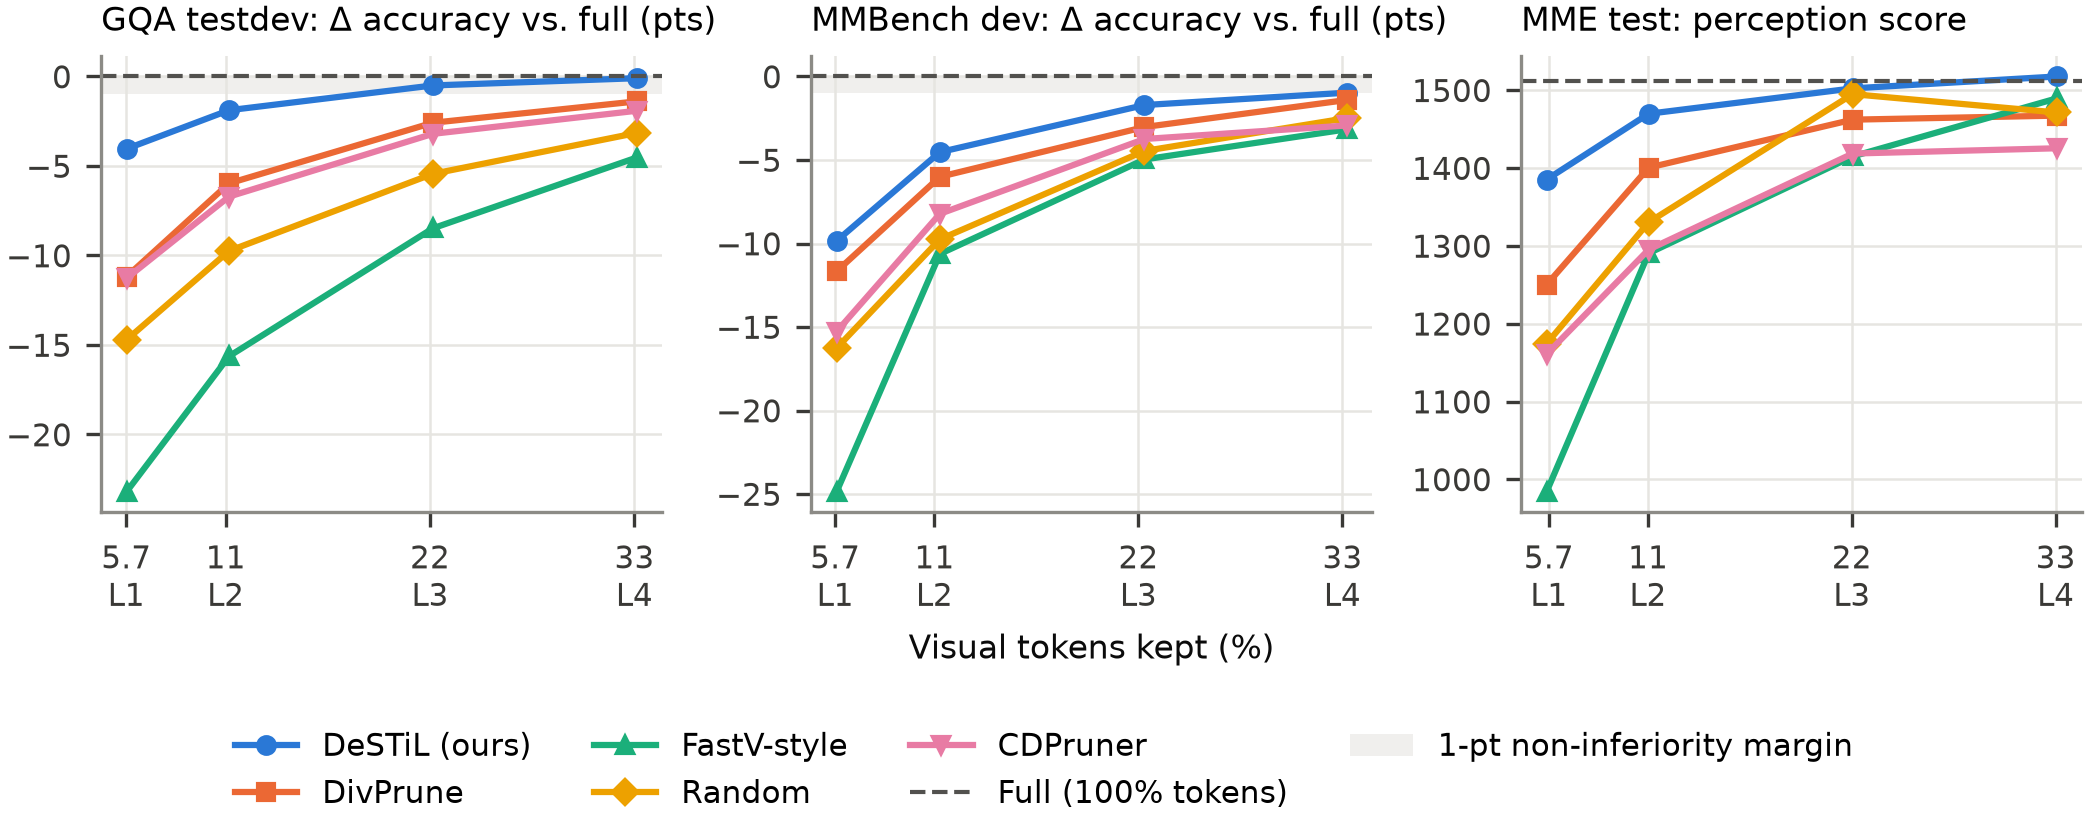
\includegraphics[width=\textwidth]{fig_budget_curves.png}
\caption{Qwen3-VL-2B: chất lượng theo tỉ lệ token giữ lại trên tập test. Dải xám: biên non-inferiority 1 điểm.}
\label{fig:budget}
\end{figure*}

So với mô hình full, DeSTiL mất \mi0,50 [\mi0,96; \mi0,05] điểm trên GQA ở L3 và \mi0,10 [\mi0,48; \pl0,29] ở L4, và đạt non-inferiority ở cả hai mức (Bảng~\ref{tab:ni}). Trên MMBench, khoảng cách lớn hơn (\mi1,71 ở L3, \mi0,97 ở L4) và không mức nào trong L1--L4 đạt non-inferiority. Ở L5 (50\%), chỉ biến thể DeSTiL-fc được chạy trên tập test; biến thể này mất \mi0,15 [\mi0,46; \pl0,16] điểm trên GQA và \mi0,21 [\mi0,69; \pl0,28] trên MMBench, đạt non-inferiority trên cả hai benchmark.

\begin{table}[!t]
\centering
\caption{Qwen3-VL-2B: non-inferiority so với mô hình full trên tập test. Mỗi ô là cận dưới một phía 95\% của hiệu số accuracy (phương pháp $-$ full, điểm \%); \ok{} nếu cận dưới $>\mi1$, tức với độ tin cậy 95\% phương pháp không kém full quá 1 điểm. Hàng L5 là biến thể DeSTiL-fc, phương pháp duy nhất được chạy ở mức này.}
\label{tab:ni}
\begin{tabular}{@{}lcc@{}}
\toprule
& GQA testdev & MMBench dev\\
\midrule
DeSTiL L2 & \mi2,34 \nok & \mi5,28 \nok\\
DeSTiL L3 & \mi0,88 \ok & \mi2,29 \nok\\
DeSTiL L4 & \mi0,42 \ok & \mi1,48 \nok\\
DeSTiL-fc L5 (50\%) & \mi0,41 \ok & \mi0,62 \ok\\
\bottomrule
\end{tabular}
\end{table}

Trên MME perception, DeSTiL cũng cao nhất ở mọi mức. Chênh lệch so với full là \mi9,2 [\mi58,1; \pl39,8] ở L3 và \pl6,1 [\mi37,8; \pl49,1] ở L4 (bootstrap theo ảnh), tức không thấp hơn có ý nghĩa thống kê, trong khi FastV-style ở L3 thấp hơn có ý nghĩa (\mi96,6 [\mi164,8; \mi24,9]). So với CDPruner, DeSTiL hơn \pl224,4 [\pl148,4; \pl298,4] ở L1 và \pl83,7 [\pl31,6; \pl136,8] ở L3. MME cognition là điểm yếu: mọi phương pháp đều giảm mạnh, và DeSTiL không dẫn đầu ở L3 và L4, nơi FastV-style cao hơn hoặc ngang. Chênh lệch của DeSTiL so với full là \mi136,4 [\mi196,3; \mi82,7] ở L3 và \mi79,6 [\mi124,8; \mi37,3] ở L4. Hình~\ref{fig:mme} cho thấy phần điểm bị mất tập trung ở các tác vụ phải đọc chữ trong ảnh; từ full sang DeSTiL L3, code\_reasoning giảm từ 108 xuống 60, text\_translation từ 185 xuống 125, numerical\_calculation từ 118 xuống 95 và OCR từ 125 xuống 118. Chữ nhỏ trải trên nhiều token nên bỏ token là mất ký tự, trong khi teacher được học trên GQA, nơi câu hỏi chủ yếu về vật thể. Ba tác vụ code\_reasoning, text\_translation và numerical\_calculation chỉ có 40 câu trên 20 ảnh mỗi tác vụ, nên một ảnh sai đã làm lệch 10--20 điểm.

\begin{figure}[!t]
\centering
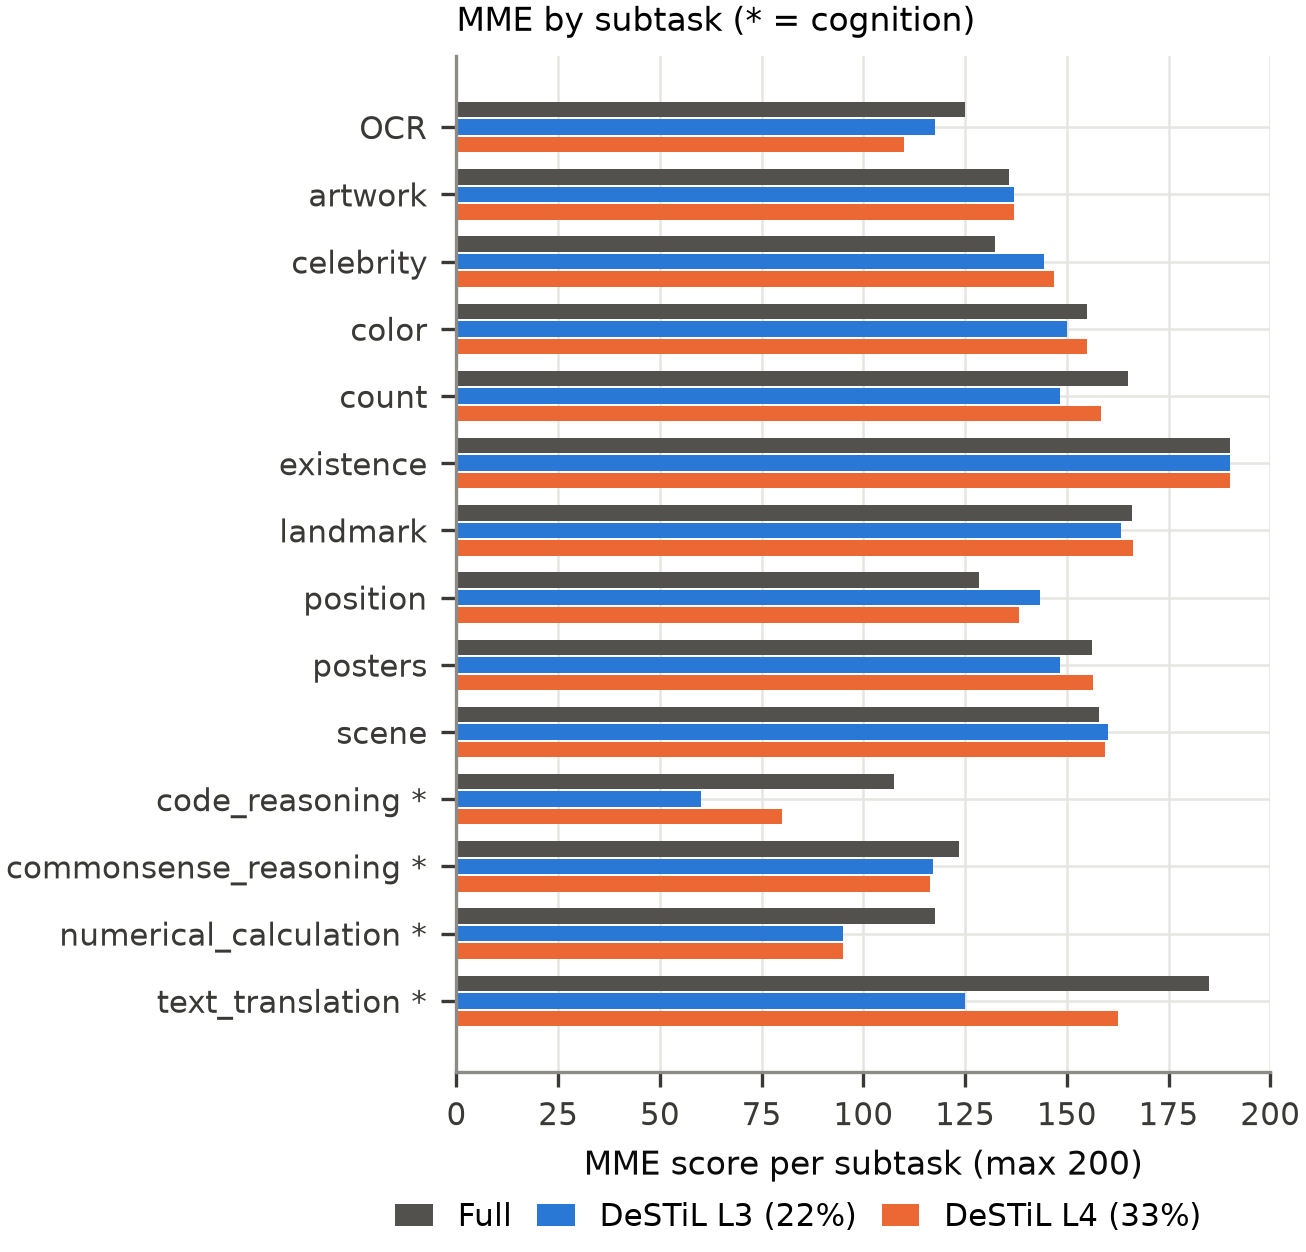
\includegraphics[width=\columnwidth]{fig_mme_subtasks.png}
\caption{Qwen3-VL-2B: điểm MME theo từng tác vụ (tối đa 200). Dấu $*$ đánh dấu tác vụ cognition.}
\label{fig:mme}
\end{figure}

\subsection{Ảo giác vật thể và suy luận khoa học}
\label{sec:pope}

POPE~\cite{li2023pope} và ScienceQA-IMG~\cite{lu2022scienceqa} được thêm sau khi cấu hình đã cố định, để kiểm tra hai điều mà GQA, MMBench và MME chưa đo trực tiếp. POPE hỏi ``Is there a \textless object\textgreater{} in the image?'' trên 500 ảnh COCO, với vật thể âm chọn ngẫu nhiên, theo tần suất (popular) hoặc theo đồng xuất hiện (adversarial); bỏ token có thể làm mô hình bỏ sót vật thể có thật hoặc khẳng định vật thể không có. ScienceQA-IMG gồm câu hỏi trắc nghiệm khoa học có ảnh, thường kèm đoạn ngữ cảnh dài. Ảnh của cả hai đều nhỏ (trung bình 269 và 171 token ảnh).

Trên POPE, DeSTiL giữ nguyên chất lượng của mô hình full từ L2: chênh lệch accuracy là \mi0,11, \pl0,18 và \pl0,06 điểm ở L2--L4 (McNemar $p\ge0{,}33$), chênh lệch F1 theo bootstrap ảnh là \pl0,12 [\mi0,57; \pl0,82], \pl0,38 [\mi0,19; \pl0,97] và \pl0,23 [\mi0,20; \pl0,70], và cận dưới một phía của chênh lệch accuracy (theo ảnh) là \mi0,62, \mi0,26 và \mi0,30. DeSTiL vì vậy đạt non-inferiority ở L2--L4 ngay cả khi tính đến việc các câu hỏi cùng ảnh không độc lập; trong các baseline, chỉ DivPrune ở L4 đạt (cận dưới \mi0,77). Ở L1, với trung bình 15 token ảnh, DeSTiL chỉ mất 1,07 điểm, so với 9,04 của DivPrune và 10,62 của CDPruner; chênh lệch ghép cặp là \pl7,98 [\pl7,19; \pl8,76] và \pl9,56 [\pl8,72; \pl10,39] điểm accuracy ($p<10^{-80}$), và \pl11,21 [\pl9,78; \pl12,83] và \pl12,25 [\pl10,53; \pl14,01] điểm F1.

Lỗi của các baseline trên POPE là bỏ sót chứ không phải bịa thêm. Ở L1, tỉ lệ trả lời ``yes'' giảm từ 45,8\% (full) xuống 29,4\% (ngẫu nhiên), 34,5\% (DivPrune) và 37,2\% (CDPruner). Precision gần như không đổi (88,5--93,9\% so với 92,9\%), còn recall giảm từ 85,1\% xuống 53,8--65,8\%: mô hình không còn thấy vật thể được hỏi nên trả lời ``no''. FastV-style là trường hợp cực đoan nhất: tỉ lệ ``yes'' chỉ còn 6,2\% ở L1 và 21,5\% ở L2, nên F1 rơi xuống 21,00 và 58,55, và mô hình thấp hơn full \mi33,69 [\mi34,80; \mi32,57] và \mi7,64 [\mi8,38; \mi6,91] điểm accuracy ở L1 và L3, kém cả chọn ngẫu nhiên ở mọi mức; attention lớp nông dồn vào token sink nên bỏ qua chính vật thể được hỏi. DeSTiL ở L1 giữ recall 84,7\% và tỉ lệ ``yes'' 46,5\%, vì score head dự đoán vùng mà LLM sẽ nhìn khi đọc tên vật thể trong câu hỏi. Đổi lại, precision của DeSTiL thấp hơn full một chút (91,1--91,7\%); trên tập adversarial, F1 của DeSTiL ở L3 là 86,92, so với 86,98 của full.

Trên ScienceQA-IMG, lợi thế của DeSTiL nhỏ hơn. DeSTiL tốt nhất ở L1--L3; so với DivPrune, DeSTiL hơn \pl1,34 [\pl0,09; \pl2,59] ở L1 ($p=0{,}043$, không còn ý nghĩa sau hiệu chỉnh Holm) và \pl1,69 [\pl0,49; \pl2,88] ở L2 ($p=0{,}007$), còn ở L3 và L4 hai phương pháp ngang nhau ($p\ge0{,}33$). So với CDPruner, DeSTiL hơn có ý nghĩa ở L1--L3 ($p\le0{,}003$), và so với FastV-style ở mọi mức (\pl4,61 [\pl3,22; \pl6,00] ở L1, \pl1,93 [\pl0,80; \pl3,07] ở L3). Không phương pháp nào đạt non-inferiority (DeSTiL L4: cận dưới \mi2,38). Chọn ngẫu nhiên ở L1 vẫn đạt 73,4\%, cho thấy nhiều câu hỏi trả lời được bằng ngữ cảnh văn bản; phần còn lại phụ thuộc vào chi tiết nhỏ của biểu đồ và hình vẽ, nơi giữ nhiều token hơn có lợi hơn là chọn đúng token, và score head chỉ được huấn luyện trên câu hỏi GQA ngắn.

\subsection{Mô hình thứ hai: Qwen3-VL-4B}
\label{sec:4b}

Để kiểm tra phương pháp có phụ thuộc vào một mô hình cụ thể hay không, toàn bộ quy trình được lặp lại trên Qwen3-VL-4B-Instruct (revision \texttt{ebb281e}, bf16). Mô hình này có cùng ViT và cùng cách bố trí token với bản 2B, nhưng LLM sâu và rộng hơn (36 lớp, chiều ẩn 2560, so với 28 lớp và 2048). Phương pháp được giữ nguyên: cùng tham số DPP và fold, cùng kiến trúc và siêu tham số của score head, cùng 50k câu hỏi GQA train làm nhãn. Chỉ hai thành phần được tính lại: bộ nén PCA (cùng kích thước đầu ra, nên head vẫn có khoảng 2 triệu tham số) và các lớp teacher (lớp 10--24 trên 36, cùng độ sâu tương đối với lớp 8--19 trên 28 của bản 2B). Checkpoint của head được chọn theo recall top-$K$ ở L3 trên các ảnh giữ lại của tập train; với bản 2B, quy tắc này chọn đúng epoch được chọn theo loss, nên mọi kết quả 2B không đổi. Cấu hình 4B được cố định trên GQA val trước khi chạy tập test, và cả năm phương pháp được chạy ở L1--L4 trên cả năm benchmark, như với bản 2B.

Phần dưới của Bảng~\ref{tab:main} cho thấy DeSTiL vẫn tốt nhất trên GQA, MMBench, POPE và MME perception ở L1--L3, với khoảng cách có ý nghĩa so với baseline mạnh nhất của từng benchmark. Trên GQA, DeSTiL hơn CDPruner \pl4,14 [\pl3,40; \pl4,89] điểm ở L1, \pl1,98 [\pl1,34; \pl2,62] ở L2 và \pl1,04 [\pl0,51; \pl1,57] ở L3 ($p\le1{,}4\cdot10^{-4}$); trên MMBench, DeSTiL hơn DivPrune \pl1,55 [\pl0,43; \pl2,67], \pl2,29 [\pl1,36; \pl3,21] và \pl1,13 [\pl0,41; \pl1,85] ($p\le0{,}008$); trên POPE, DeSTiL hơn CDPruner \pl3,18 [\pl2,08; \pl4,26] điểm ở L1 và \pl1,11 [\pl0,31; \pl1,88] ở L2 (bootstrap theo ảnh). Trên MME perception, DeSTiL hơn CDPruner \pl92,0 [\pl29,3; \pl160,0] ở L1 và \pl96,0 [\pl36,4; \pl152,4] ở L2, và hơn DivPrune \pl94,4 [\pl49,3; \pl144,1] ở L3. Ở L4 (33,4\%), các phương pháp tiến sát nhau: DeSTiL vẫn có điểm cao nhất trên GQA, POPE và MME perception, nhưng chênh lệch so với baseline mạnh nhất không còn ý nghĩa (GQA \pl0,43 so với CDPruner, $p=0{,}068$; POPE \pl0,17, $p=0{,}33$; MME perception \pl27,1 [\mi14,3; \pl73,7] so với DivPrune), và trên MMBench DeSTiL ngang DivPrune (\mi0,05, $p=0{,}94$). POPE L3 so với CDPruner (\pl0,23, $p=0{,}23$) cũng không có ý nghĩa. Thứ hạng của các baseline thủ công không ổn định giữa hai mô hình: trên 4B, CDPruner hơn DivPrune trên GQA và POPE ở mọi mức nhưng kém hơn trên MMBench, trong khi trên 2B CDPruner kém DivPrune ở cả GQA và MMBench.

So với chọn ngẫu nhiên, DeSTiL hơn có ý nghĩa trên GQA và POPE ở mọi mức (GQA \pl11,36 [\pl10,51; \pl12,21] ở L1 và \pl2,46 [\pl1,89; \pl3,02] ở L4; POPE \pl12,92 và \pl2,48), trên MMBench ở L1--L3 (\pl1,92 đến \pl3,07, $p\le6\cdot10^{-6}$) và trên MME perception ở L1--L3 (\pl119,5 đến \pl157,0); ở L4, chênh lệch trên MMBench (\pl0,58, $p=0{,}13$) và MME perception (\pl40,3 [\mi12,0; \pl91,8]) không còn ý nghĩa. FastV-style lặp lại hành vi trên 2B: kém hơn chọn ngẫu nhiên trên GQA, MMBench và POPE ở mọi mức, và trên POPE tỉ lệ ``yes'' chỉ còn 13,3\% ở L1 (full 44,2\%, DeSTiL 43,3\%), nên DeSTiL hơn FastV-style \pl25,21 [\pl24,18; \pl26,25] điểm accuracy ở L1 và \pl3,50 [\pl2,95; \pl4,05] ở L4. Trên ScienceQA-IMG, DeSTiL có accuracy cao nhất ở L1, L2 và L4, và hơn DivPrune và CDPruner có ý nghĩa ở mọi mức (\pl1,34 đến \pl2,43, $p\le0{,}05$). FastV-style là đối thủ gần nhất trên benchmark này: ở L3 nó cao hơn DeSTiL (86,27 so với 85,97; \mi0,30 [\mi1,63; \pl1,03] theo hướng DeSTiL trừ FastV-style), và ở L2 và L4 chênh lệch không có ý nghĩa ($p=0{,}07$ và $0{,}69$). Khoảng cách với full trên ScienceQA-IMG lớn hơn bản 2B (DeSTiL \mi12,35 ở L1 và \mi5,16 ở L4, so với \mi6,79 và \mi1,54 trên 2B): full 4B đạt 92,56\%, cao hơn full 2B gần 6 điểm, nhưng DeSTiL ở L1 trên hai mô hình chỉ chênh 0,35 điểm (80,22 so với 79,87), tức phần lợi của mô hình lớn hơn trên benchmark này nằm chủ yếu ở các token bị bỏ. Điều này nhất quán với nhận xét ở Mục~\ref{sec:pope} rằng benchmark này phụ thuộc vào chi tiết nhỏ của hình vẽ, nơi số token giữ lại quan trọng hơn việc chọn đúng token.

So với mô hình full, DeSTiL đạt non-inferiority trên POPE ở L3 (\mi0,24; cận dưới một phía \mi0,62 theo ảnh) và L4 (\mi0,19; cận dưới \mi0,56), và chênh lệch trên MME perception ở L3 (\mi8,7 [\mi59,8; \pl42,2]) và L4 (\mi17,5 [\mi62,5; \pl21,7]) không khác 0. Trên GQA, DeSTiL mất \mi1,23 điểm ở L3 và \mi0,76 ở L4; cận dưới ở L4 là \mi1,09, sát nhưng chưa qua biên 1 điểm. Trên MMBench, khoảng cách là \mi2,26 ở L3 và \mi1,82 ở L4. Các khoảng cách này lớn hơn bản 2B. Recall top-$K$ của head 4B trên ảnh giữ lại là 0,757, so với 0,836 của bản 2B, trong khi điểm thủ công đạt 0,31 và 0,30: teacher 4B tập trung hơn (khối lượng attention của token cao nhất 0,15 so với 0,066) nên khó bắt chước hơn với cùng lượng nhãn. Trên MME cognition, DivPrune cao nhất ở L1, L3 và L4 (415,4, 525,0 và 545,0, so với 353,9, 481,4 và 508,6 của DeSTiL), chọn ngẫu nhiên cũng cao hơn DeSTiL ở L1 (384,6) và FastV-style ở L4 (540,7), còn DeSTiL chỉ dẫn đầu ở L2 (422,1 so với 412,9), giống với bản 2B: các tác vụ đọc chữ và code cần nhiều token trải đều trên ảnh, mà một bộ chọn đa dạng giữ được nhiều hơn.

\subsection{Phát triển, xác nhận và ablation}
\label{sec:ablation}

Cấu hình được chọn trên tune2k và chốt trước khi chấm tập xác nhận gqa\_val\_confirm, nơi baseline chỉ được chạy ở L1 và L3 (Bảng~\ref{tab:dev}). Trên tập xác nhận, DeSTiL hơn DivPrune \pl9,84 [\pl8,55; \pl11,12] ở L1 và \pl2,92 [\pl2,09; \pl3,76] ở L3, và hơn FastV-style \pl6,85 [\pl5,76; \pl7,94] ở L3 (McNemar, tất cả $p<0{,}001$). Ở các mức có đủ số liệu, ba tập tune2k, confirm và testdev cho cùng thứ hạng.

\begin{table}[!t]
\centering
\caption{Qwen3-VL-2B: chênh lệch so với full trên GQA val. tune2k: $n=2000$, full 68,90\%. confirm: $n=4890$, không trùng tune2k, full 69,55\%. LB: cận dưới một phía. ``--'': không chạy.}
\label{tab:dev}
\setlength{\tabcolsep}{4pt}
\begin{tabular}{@{}lccccc@{}}
\toprule
& Ngẫu nhiên & DivPrune & FastV-st. & DeSTiL & LB DeSTiL\\
\midrule
\multicolumn{6}{@{}l}{\emph{tune2k}}\\
L1 & \mi20,10 & \mi16,55 & \mi30,40 & \best{\mi4,35} & \\
L2 & \mi13,05 & \mi7,90 & \mi17,85 & \best{\mi1,20} & \\
L3 & \mi6,95 & \mi3,35 & \mi7,70 & \best{\mi0,20} & \\
L4 & \mi4,00 & \mi1,45 & \mi4,35 & \best{\mi0,20} & \\
\midrule
\multicolumn{6}{@{}l}{\emph{gqa\_val\_confirm}}\\
L1 & \mi18,69 & \mi14,46 & \mi29,08 & \best{\mi4,62} & \mi5,45\\
L2 & -- & -- & -- & \mi1,62 & \mi2,30\\
L3 & \mi5,81 & \mi3,11 & \mi7,03 & \best{\mi0,18} & \mi0,73 \ok\\
L4 & -- & -- & -- & \pl0,04 & \mi0,43 \ok\\
\bottomrule
\end{tabular}
\end{table}

Bảng~\ref{tab:ablation} liệt kê chênh lệch so với full của từng cấu hình trên tune2k, và Hình~\ref{fig:ablation} vẽ năm cấu hình chính theo bốn mức budget, sắp theo thứ tự thêm từng thành phần: chọn ngẫu nhiên, DPP với điểm cosine của CDPruner, DPP với điểm thủ công của DSFold-D, rồi score head học từ gradient và từ teacher. Cột của hai score head ngắn hơn hẳn các cột còn lại ở mọi mức, tức trọng số chất lượng học được là bước tiến lớn nhất. Ở cùng DPP và fold, thay điểm thủ công của DSFold-D bằng score head tăng \pl6,70 [\pl4,74; \pl8,66] điểm ở L1 và \pl3,05 [\pl1,70; \pl4,40] ở L3 (cả hai $p<10^{-4}$), và so với CDPruner, DeSTiL hơn \pl12,60 ở L1 và \pl4,80 ở L3 (cả hai $p<10^{-9}$). Lợi ích vì vậy đến từ trọng số học được chứ không chỉ từ DPP có điều kiện. Ngay cả điểm thủ công của DSFold-D (cosine lớn nhất theo từng từ, chuẩn hóa z, cộng saliency DeepStack) cũng hơn cosine với embedding trung bình của CDPruner \pl5,90 ở L1 và \pl1,75 ở L3, và hơn DivPrune ở L1, L2, L4 (ngang ở L3, $p=0{,}95$). Về nguồn nhãn, với 10k nhãn, \Htg{} học từ teacher hơn \Hmlp{} học từ gradient \pl1,70 [\pl0,60; \pl2,80] ở L3 ($p=0{,}003$) nhưng chỉ \pl0,25 ở L4 ($p=0{,}68$); so sánh này đổi cả nguồn nhãn lẫn kiến trúc nên không tách được hai yếu tố. Với 50k nhãn, DeSTiL kém \Hmlp-grad 1,20 điểm ở L1 ($p=0{,}15$) và hơn \pl0,20--\pl0,40 ở L2--L4, tức nhãn teacher không cần lượt backward và cho kết quả ít nhất tương đương. Fold DeepStack không tạo khác biệt đo được trên GQA.

\begin{table}[!t]
\centering
\caption{Qwen3-VL-2B: ablation trên tune2k (chênh lệch so với full, điểm \%). ``grad'': nhãn saliency gradient; ``teacher'': nhãn attention. Số trong ngoặc là số nhãn huấn luyện.}
\label{tab:ablation}
\setlength{\tabcolsep}{3.5pt}
\begin{tabular}{@{}lcccc@{}}
\toprule
Cấu hình & L1 & L2 & L3 & L4\\
\midrule
Ngẫu nhiên (có fold) & \mi20,10 & \mi13,05 & \mi6,95 & \mi4,00\\
DivPrune & \mi16,55 & \mi7,90 & \mi3,35 & \mi1,45\\
CDPruner: DPP, cosine TB & \mi16,95 & \mi9,65 & \mi5,00 & \mi2,75\\
DSFold-D: DPP, điểm thủ công & \mi11,05 & \mi6,05 & \mi3,25 & \mi0,95\\
\midrule
\Hmlp, grad (10k) & & & \mi1,95 & \mi0,45\\
\Hmlp, grad (50k) & \mi3,15 & \mi1,60 & \mi0,50 & \mi0,40\\
\Hattn, grad (50k) & & & \mi1,00 & \mi0,70\\
\Htg, teacher (10k) & & & \mi0,25 & \mi0,20\\
\textbf{\Htg, teacher (50k) = DeSTiL} & \mi4,35 & \mi1,20 & \mi0,20 & \mi0,20\\
DeSTiL không fold ($\gamma=0$) & & \mi1,25 & \mi0,25 & \pl0,15\\
\bottomrule
\end{tabular}
\end{table}

\begin{figure}[!t]
\centering
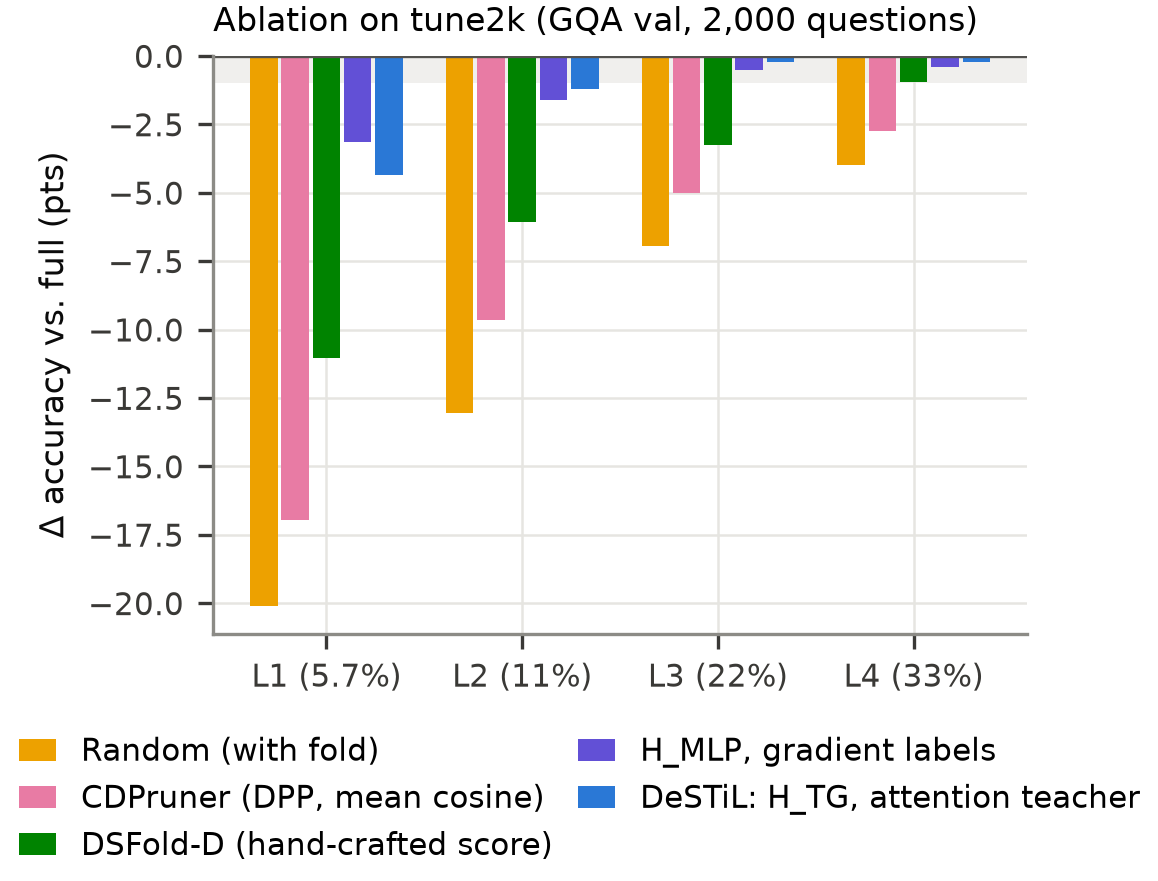
\includegraphics[width=\columnwidth]{fig_ablation.png}
\caption{Qwen3-VL-2B: ablation trên tune2k (chênh lệch so với full, điểm \%).}
\label{fig:ablation}
\end{figure}

\subsection{Phân tích token được chọn}
\label{sec:region}

Hình~\ref{fig:examples} so sánh tập token giữ lại của bốn bộ chọn trên cùng một ảnh. Ở hàng (a), với câu ``Which kind of device does the boy play with?'', DeSTiL giữ cụm token ở tay và cái điều khiển nên trả lời ``wii controller'', còn các phương pháp khác chỉ nói được ``controller''; ở câu thứ hai, DeSTiL giữ các token ở cửa sổ và rèm, còn DivPrune rải token khắp phòng và FastV-style dồn token vào các vùng sáng đồng nhất. Hàng (b) của Hình~\ref{fig:examples} cho thấy hai kiểu lỗi. Kiểu thứ nhất là thiếu chi tiết nhỏ: DeSTiL giữ token ở khuôn mặt và áo cậu bé nhưng bỏ phần lớn chiếc bánh trên đĩa, nên đoán ``pizza'' thay vì ``hamburger''. Kiểu thứ hai là câu hỏi so sánh hai đối tượng: với câu hỏi cái bàn hay cái giường không sạch, DeSTiL tập trung vào giường mà bỏ mặt bàn, trong khi DivPrune nhờ phủ đều nên giữ được cả hai.

\begin{figure*}[!t]
\centering
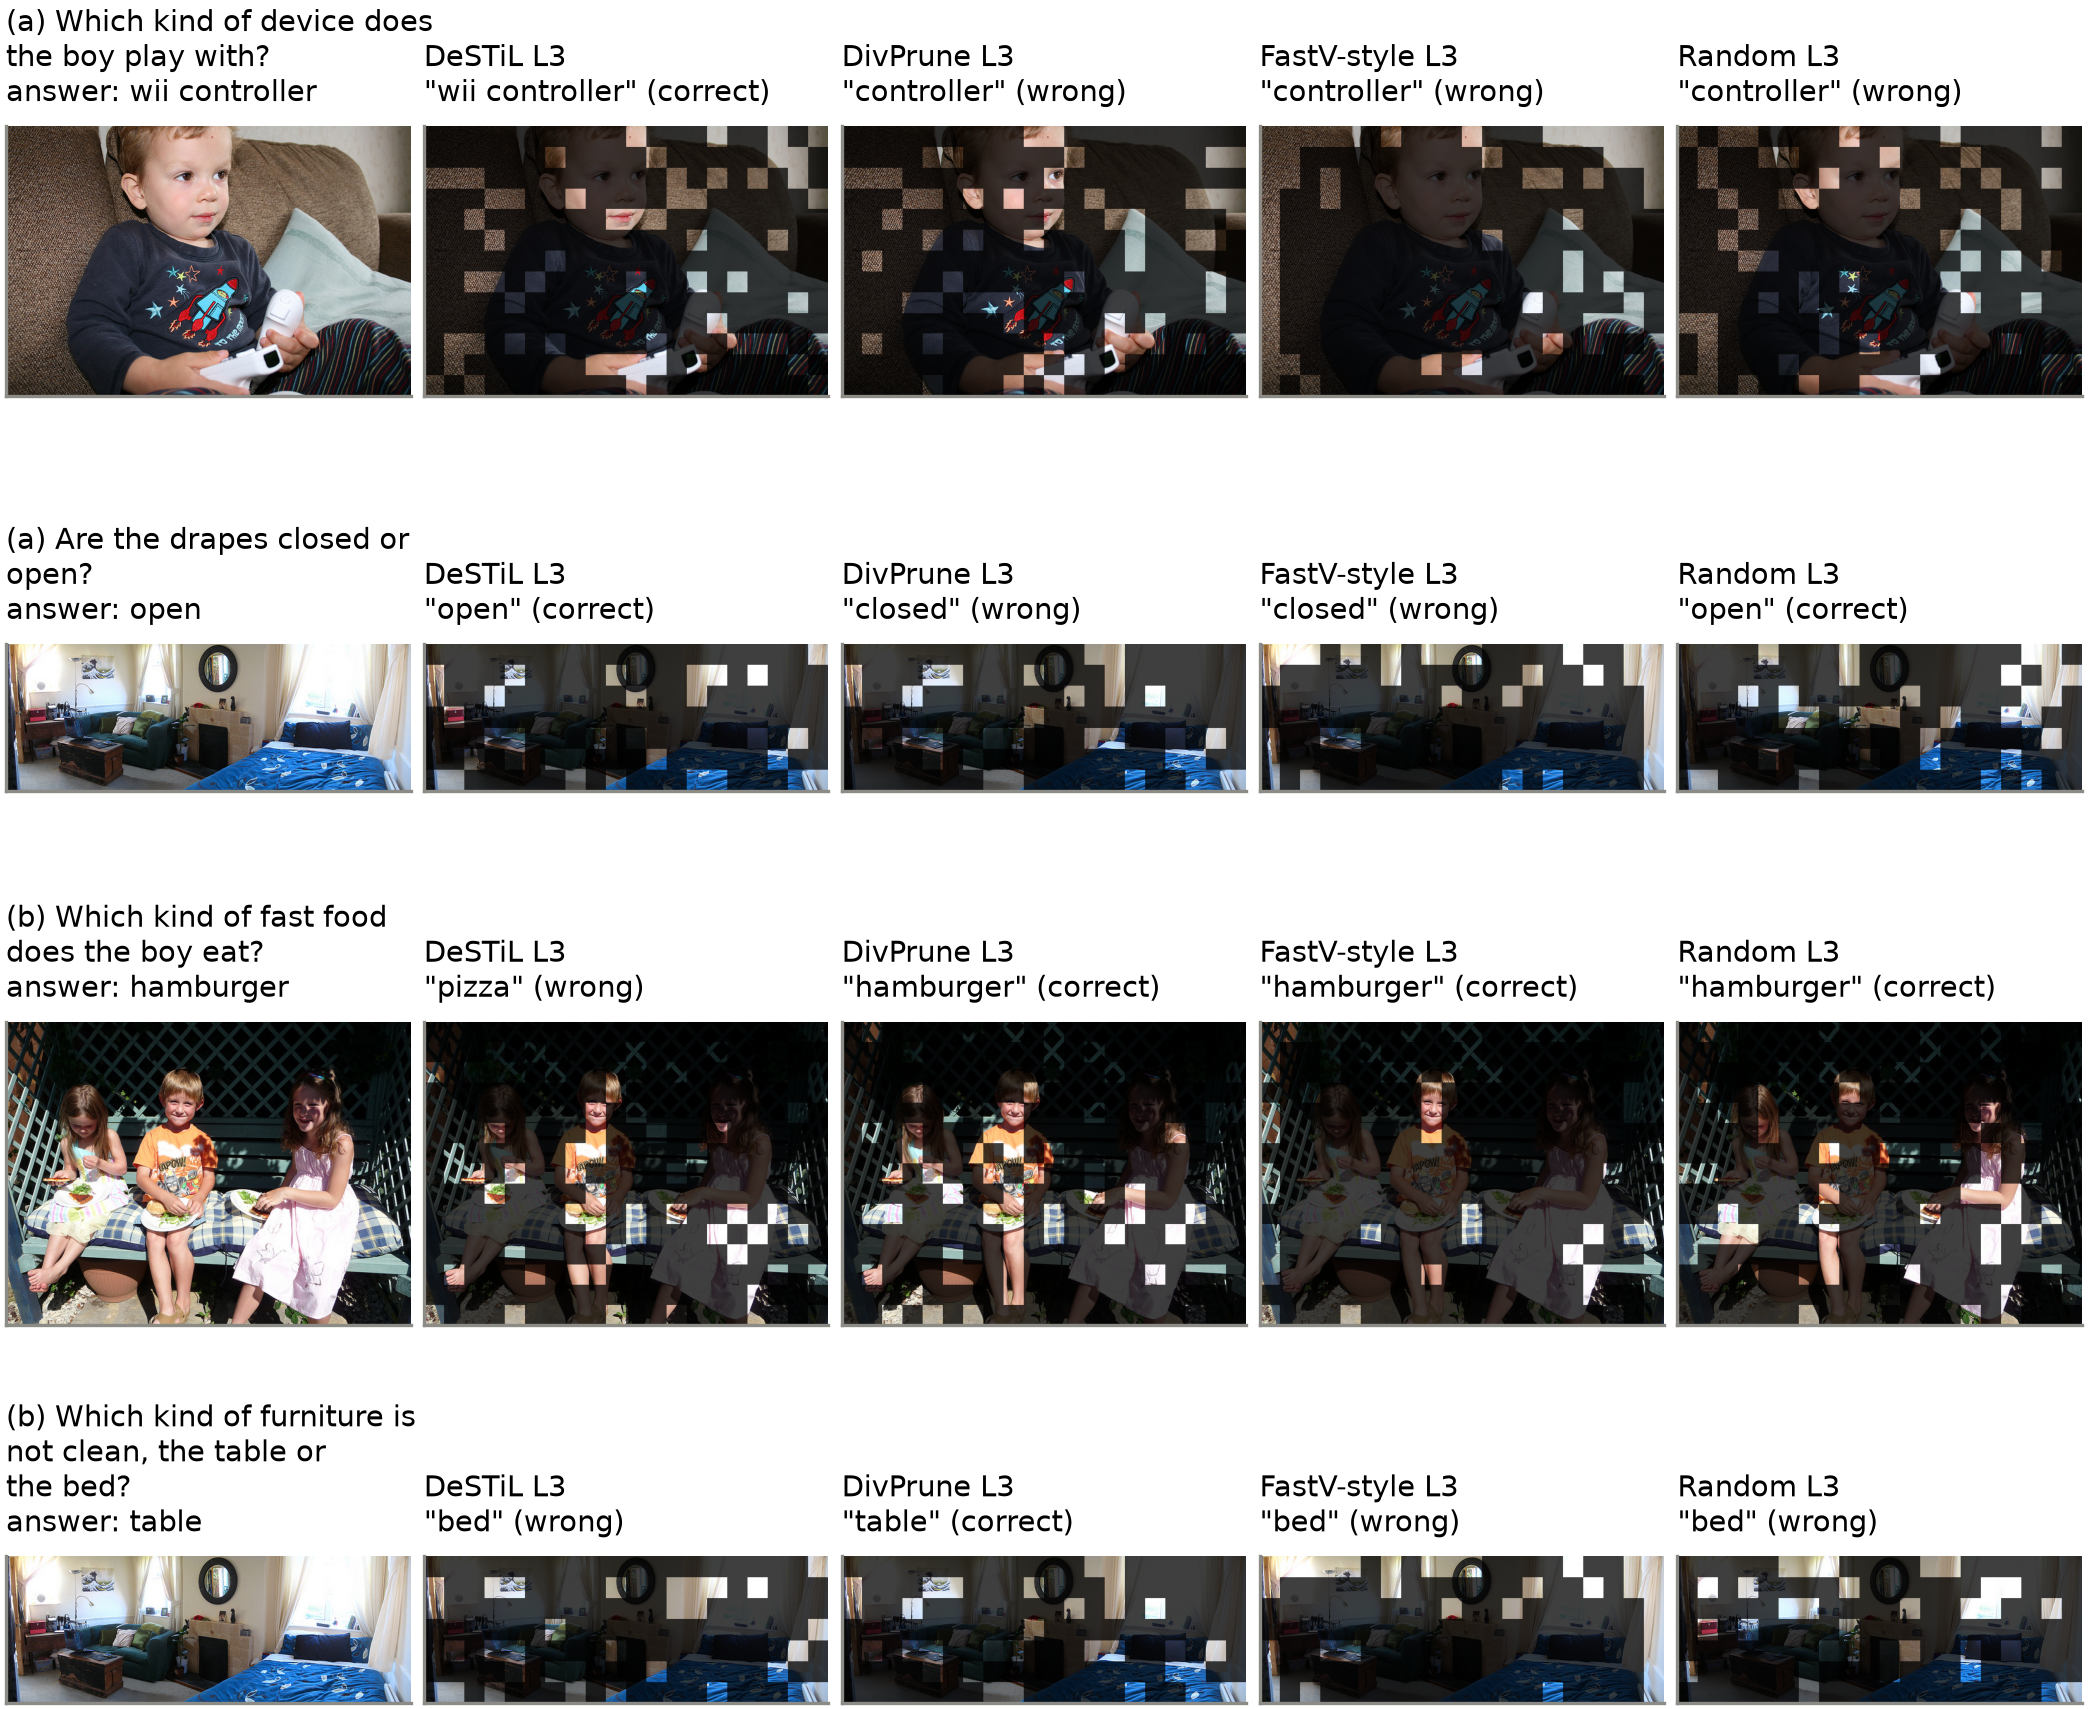
\includegraphics[width=\textwidth]{fig_selection.png}
\caption{Token giữ lại (sáng) và bị bỏ (tối) ở budget 22\% trên GQA testdev. Ví dụ được chọn theo thứ tự mã câu hỏi trong các câu không phải yes/no, $120\le N\le300$, mỗi ảnh một câu, mà mô hình full trả lời đúng. (a) Hai câu đầu tiên mà DeSTiL đúng còn DivPrune và FastV-style sai. (b) Hai câu đầu tiên mà DeSTiL sai còn DivPrune đúng.}
\label{fig:examples}
\end{figure*}

Để đo hình dạng vùng, với tập giữ lại $S$ trên lưới $H'\times W'$, \emph{số vùng trên 10 token} là $10\cdot C(S)/|S|$, với $C(S)$ là số thành phần liên thông 8 hướng của $S$, và \emph{mức trùng giữa câu hỏi} là trung bình Jaccard $|S_a\cap S_b|/|S_a\cup S_b|$ trên mọi cặp câu hỏi khác nhau của cùng một ảnh, rồi trung bình theo ảnh. Theo nửa dưới của Hình~\ref{fig:region}, DeSTiL gắn với ảnh nhiều hơn với câu hỏi: mức trùng là 0,65, 0,72 và 0,81 ở L3, L4 và L5, gấp nhiều lần chọn ngẫu nhiên, là dấu vết của attention sink mà head học từ teacher. Ở cùng số token, DeSTiL-fc giảm mức trùng của toàn tập giữ lại xuống 0,61 ở L4 (so với 0,72) và 0,72 ở L5 (so với 0,81). Phần focus của DeSTiL-fc (8,5--12,5\% token) gọn (1,4--1,8 vùng trên 10 token) và ít trùng (0,15--0,18), dù hai con số này đo trên một tập nhỏ hơn nên không so trực tiếp được với DeSTiL. Accuracy không đổi: ở L5 trên tune2k, DeSTiL-fc đạt 68,85\% so với 68,70\% của DeSTiL; ở L4, tỉ lệ focus 0, 25, 40 và 55\% cho chênh lệch \mi0,20, \mi0,35, \mi0,60 và \mi1,05 điểm. Nửa trên của Hình~\ref{fig:region} minh họa: câu về con vật té nước tập trung vào nước quanh con chó, câu về mặt nước tập trung vào mặt nước, câu về con chó tập trung vào thân con chó.

\begin{figure*}[!t]
\centering
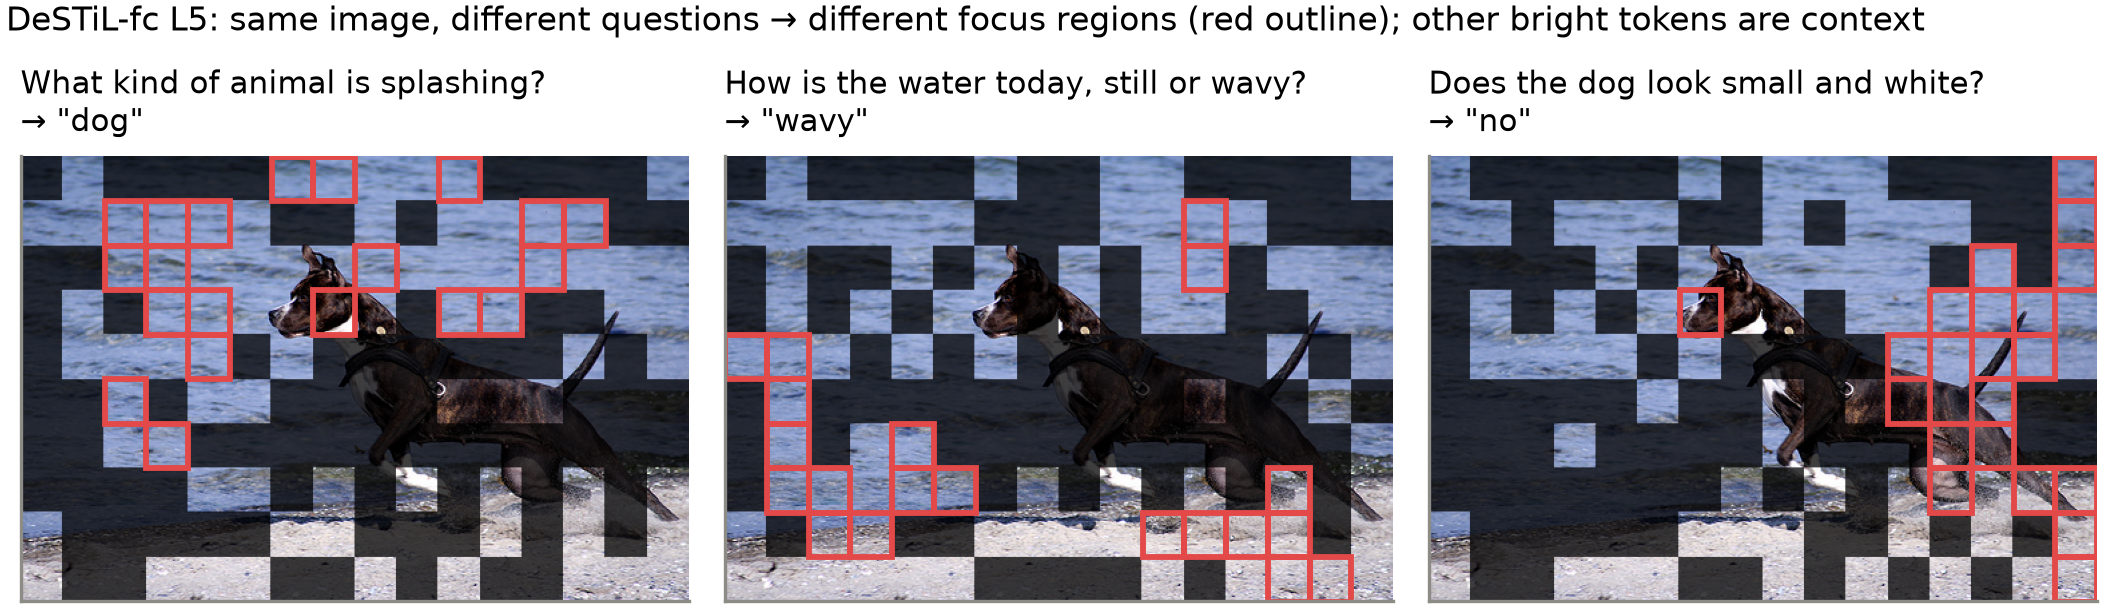
\includegraphics[width=\textwidth]{fig_focus_questions.png}\\[4pt]
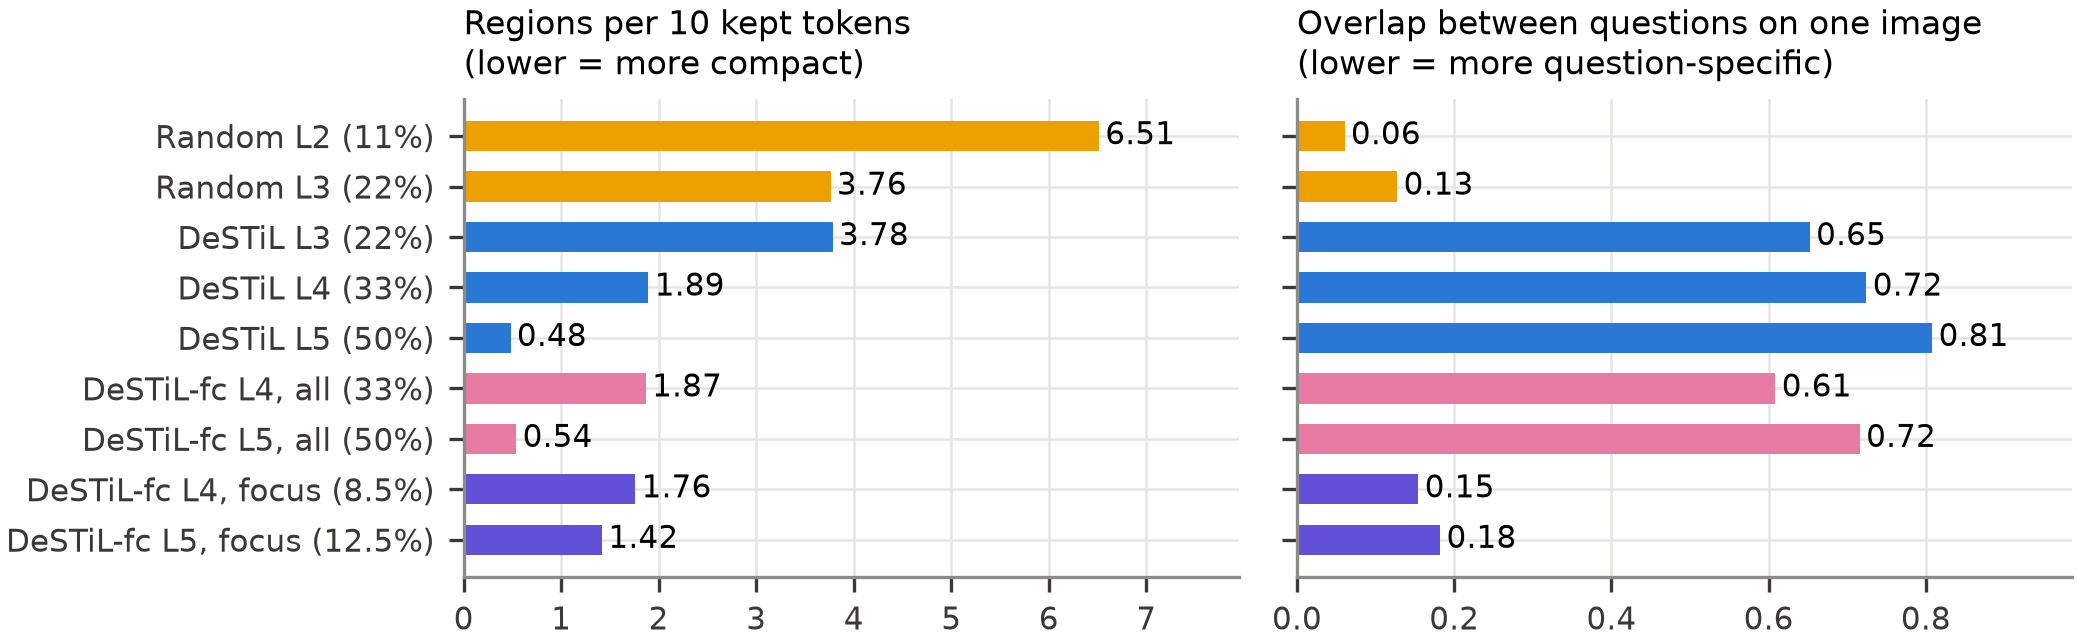
\includegraphics[width=\textwidth]{fig_region.png}
\caption{Hình dạng và mức phụ thuộc câu hỏi của tập token giữ lại. Trên: DeSTiL-fc ở L5, cùng một ảnh với ba câu hỏi khác nhau cho ba vùng focus (viền đỏ) khác nhau; phần sáng còn lại là context. Dưới: trên tune2k, số vùng rời nhau trên 10 token giữ lại (trái, thấp = gọn) và mức trùng Jaccard giữa các câu hỏi trên cùng ảnh (phải, thấp = phụ thuộc câu hỏi).}
\label{fig:region}
\end{figure*}

Câu yes/no (566 trên 2000 câu của tune2k) vẫn thấp hơn full 0,7--1,8 điểm ở mọi budget tới 50\%, dù có hay không có fold. Lỗi chủ yếu là câu có đáp án ``no'' bị trả lời ``yes'': ở L4, 14 câu ``no'' bị mất và 1 câu được thêm, còn 3 câu ``yes'' bị mất và 6 câu được thêm. Chọn ngẫu nhiên thì ngược lại, chủ yếu mất câu ``yes'' (24 câu). Một giả thuyết là khi chỉ giữ token quanh đối tượng được hỏi, mô hình thiếu bằng chứng để phủ định.

\subsection{Hiệu năng}
\label{sec:timing}

Phép đo dùng một tiến trình riêng trên GPU, 300 câu mỗi tập: 300 câu đầu của tune2k (GQA, $\bar N=223$) và 300 câu đầu của MME test (code\_reasoning và artwork, $\bar N=877$, ít hơn trung bình 1756 của toàn bộ MME test). Với mỗi câu, thứ tự chạy các cấu hình được xáo ngẫu nhiên. Bộ giải DPP tham lam và max--min được chạy bằng CUDA graph, 16 bước mỗi lần phát lại (với $K\ge48$); tập token giữ lại trùng với bản từng bước ở 2099 trên 2100 cặp (câu, cấu hình) của MME, nên mọi kết quả chất lượng ở trên không đổi. FLOPs được tính giải tích cho decoder của LLM (Phụ lục~\ref{app:flops}).

Về FLOPs, cắt token có lợi rõ (Bảng~\ref{tab:timing}). Ở L3, FLOPs prefill giảm 3,3 lần trên GQA và 4,1 lần trên MME, và ở L1 trên MME giảm 10,9 lần; trên toàn bộ MME test ($\bar N=1756$), DeSTiL L3 giảm FLOPs prefill 5,2 lần và DeSTiL L1 giảm 16,9 lần. Bộ chọn của DeSTiL (score head và DPP) chỉ tốn 1,3~GFLOPs trên GQA và 8,4~GFLOPs trên MME, dưới 1,3\% FLOPs prefill của mô hình full.

\begin{table*}[!t]
\centering
\caption{Qwen3-VL-2B: hiệu năng ở batch 1: token ảnh $K$ / token vào LLM, FLOPs prefill của LLM (cộng bộ chọn), thời gian chọn token và prefill (ms, trung vị), tổng chọn + prefill (trung vị [IQR]) và hệ số tăng tốc so với full. ViT (trung vị 33~ms trên GQA, 152~ms trên MME) và decode giống nhau cho mọi phương pháp, không tính vào cột tổng.}
\label{tab:timing}
\setlength{\tabcolsep}{3pt}
\footnotesize
\begin{tabular}{@{}lccccc|ccccc@{}}
\toprule
& \multicolumn{5}{c|}{GQA, 300 câu tune2k ($\bar N=223$)} & \multicolumn{5}{c}{MME, 300 câu ($\bar N=877$)}\\
& $K$ / vào LLM & TFLOPs ($\times$) & chọn & prefill & chọn + prefill ($\times$) & $K$ / vào LLM & TFLOPs ($\times$) & chọn & prefill & chọn + prefill ($\times$)\\
\midrule
Full & 192 / 215 & 0,71 (1,0) & -- & 30,4 & 30,5 [29,3; 34,8] (1,00) & 880 / 914 & 2,69 (1,0) & -- & 84,3 & 84,4 [68,3; 107,3] (1,00)\\
Ngẫu nhiên L3 & 43 / 66 & 0,21 (3,3) & 2,6 & 27,9 & 30,5 [29,7; 32,9] (1,00) & 196 / 230 & 0,66 (4,1) & 2,8 & 30,9 & 34,0 [31,9; 38,4] (2,48)\\
DivPrune L3 & 43 / 66 & 0,21 (3,3) & 6,8 & 27,9 & 34,8 [33,5; 43,3] (0,88) & 196 / 230 & 0,66 (4,1) & 26,7 & 31,3 & 57,6 [52,1; 69,4] (1,46)\\
CDPruner L3 & 43 / 66 & 0,21 (3,3) & 13,4 & 28,1 & 41,4 [39,7; 45,0] (0,74) & 196 / 230 & 0,66 (4,1) & 18,1 & 34,1 & 52,0 [47,1; 59,7] (1,62)\\
DeSTiL L1 & 11 / 36 & 0,11 (6,5) & 9,6 & 28,3 & 37,9 [36,9; 45,6] (0,80) & 50 / 83 & 0,25 (10,9) & 19,4 & 29,0 & 48,4 [45,7; 51,6] (1,75)\\
DeSTiL L3 & 43 / 66 & 0,21 (3,3) & 17,8 & 28,2 & 45,8 [44,0; 49,4] (0,67) & 196 / 230 & 0,66 (4,1) & 23,1 & 32,4 & 55,3 [51,5; 61,6] (1,53)\\
DeSTiL L4 & 64 / 87 & 0,29 (2,5) & 17,5 & 29,2 & 46,7 [45,5; 55,0] (0,65) & 294 / 327 & 0,95 (2,8) & 26,2 & 38,8 & 64,7 [58,6; 77,2] (1,31)\\
\bottomrule
\end{tabular}
\end{table*}

Về thời gian (Bảng~\ref{tab:timing}; phân rã theo từng bước ở Phụ lục~\ref{app:timing}), lợi ích phụ thuộc vào số token ảnh. Trên MME, tổng chọn + prefill của DeSTiL giảm từ 84,4~ms xuống 48,4~ms ở L1 (1,75 lần), 55,3~ms ở L3 (1,53 lần) và 64,7~ms ở L4 (1,31 lần); DeSTiL L3 nhanh hơn DivPrune L3 (57,6~ms) và chỉ chậm hơn CDPruner L3 3,3~ms dù có thêm score head. Tính cả ViT và decode, trung vị thời gian mỗi câu MME của DeSTiL L3 giảm từ 265 xuống 234~ms (1,13 lần), bằng DivPrune L3 và CDPruner L3, vì ViT chiếm phần lớn thời gian còn lại. Trên GQA, không phương pháp nào nhanh hơn full: prefill gần như không đổi theo số token (30,4~ms với 215 token so với 27,9~ms với 66 token), vì ở batch 1 với vài trăm token, prefill bị giới hạn bởi số lần gọi kernel chứ không phải số phép tính. Khi đó mọi bộ chọn có chi phí đều làm tổng thời gian tăng, và DeSTiL tốn thêm 15~ms ở L3. Bộ nhớ đỉnh giảm tối đa khoảng 0,15~GB trên MME, vì trọng số mô hình chiếm phần lớn. Trên Qwen3-VL-4B, tăng tốc lớn hơn vì LLM tốn hơn trên mỗi token còn bộ chọn gần như không đổi: trên MME, chọn token + prefill của DeSTiL tốn 113~ms ở L1 và 254~ms ở L3, so với 644~ms prefill của mô hình full (nhanh hơn 5,7 và 2,5 lần).

% ======================================================================
\section{Thảo luận}
\label{sec:discussion}
Lợi ích của DeSTiL đến từ trọng số chất lượng học được, không phải từ bộ giải DPP. Ở cùng DPP và fold, thay điểm thủ công bằng score head tăng 3--7 điểm trên tập phát triển (Mục~\ref{sec:ablation}), và recall top-$K$ so với teacher tăng từ 0,30 lên 0,84. Điểm thủ công, là cosine giữa token ảnh và câu hỏi, chỉ đo token ``giống'' câu hỏi tới đâu trong không gian embedding; score head học được những token mà LLM thật sự dùng ở các lớp giữa, kể cả ngữ cảnh xung quanh đối tượng. So sánh với CDPruner trên tập test xác nhận kết luận này với một DPP có điều kiện đã công bố: cùng dạng kernel và cùng bộ giải, DeSTiL hơn CDPruner 1,8--7,2 điểm trên GQA testdev với Qwen3-VL-2B và 0,4--4,1 điểm với Qwen3-VL-4B (Bảng~\ref{tab:main}).

Thứ hạng của các baseline thủ công thay đổi theo mô hình và benchmark, trong khi DeSTiL giữ vị trí dẫn đầu. Trên 2B, DivPrune hơn CDPruner trên GQA và MMBench; trên 4B, CDPruner hơn DivPrune trên GQA và POPE nhưng kém hơn trên MMBench. Mỗi tiêu chí thủ công (đa dạng thuần túy, hay liên quan theo cosine) chỉ phù hợp với một kiểu câu hỏi, còn tín hiệu attention được chưng cất phản ánh trực tiếp nhu cầu của LLM trên từng cặp ảnh--câu hỏi, nên DeSTiL tốt nhất trên GQA, MMBench, POPE và MME perception ở cả hai mô hình từ 5,7\% đến 22,4\% token. Hành vi trên POPE minh họa rõ cơ chế này: các baseline giữ precision nhưng mất recall vì bỏ token của vật thể được hỏi, còn DeSTiL giữ gần như nguyên recall và tỉ lệ trả lời ``yes'' của mô hình full (Mục~\ref{sec:pope}).

Attention ở lớp nông không phải là tín hiệu thay thế tốt cho attention ở lớp giữa. FastV-style, chọn token theo attention ở lớp 2, kém hơn chọn ngẫu nhiên trên GQA, MMBench và POPE ở mọi mức trên cả hai mô hình, vì attention ở lớp này dồn vào các token sink ở vùng sáng và nền đồng nhất. Trên MME, FastV-style cao hơn chọn ngẫu nhiên ở perception L4 (1489,4 so với 1471,5) và ở cognition L1, L3, L4, phù hợp với việc attention lớp nông vẫn tìm được vùng chữ có tương phản cao. DeSTiL lấy nhãn từ attention ở các lớp giữa (lớp 8--19 trên 28 của bản 2B) thay vì lớp 2, và kết hợp trọng số này với thành phần đa dạng của DPP, nên một tập token giữ lại không bị chiếm bởi token sink; việc chọn vẫn diễn ra trước LLM, tương thích với FlashAttention.

Ở budget lớn, DeSTiL tiến sát mô hình full. Trên MME perception, DeSTiL ở L4 không thấp hơn full; trên POPE, DeSTiL ở L3 cao hơn full \pl0,18 điểm accuracy và \pl0,38 điểm F1, với khoảng tin cậy chứa 0. Vì score head được huấn luyện để bắt chước attention của chính mô hình full, mô hình full là mức trần tự nhiên của phương pháp, và kết quả ở L3--L4 cho thấy DeSTiL đạt gần mức trần này với một phần ba số token ảnh.

% ======================================================================
\section{Kết luận}
Thay điểm liên quan thủ công trong DPP có điều kiện bằng một score head 2 triệu tham số, chưng cất từ attention văn bản$\rightarrow$ảnh của chính LLM, cho một bộ chọn token ảnh mạnh trên mô hình DeepStack Qwen3-VL-2B. Ở cùng budget, DeSTiL tốt hơn chọn ngẫu nhiên, DivPrune, FastV-style và CDPruner trên GQA, MMBench và MME perception, với khoảng cách lớn nhất ở budget nhỏ nhất. Với 22--33\% token ảnh, DeSTiL đạt non-inferiority trên GQA, và không thấp hơn có ý nghĩa trên MME perception. Trên POPE, DeSTiL đạt non-inferiority từ 11\% token, và ở 5,7\% token giữ được recall gần như của mô hình full, trong khi các baseline bỏ sót vật thể được hỏi. Chạy bằng CUDA graph, bộ chọn chỉ tốn khoảng 20~ms; trên ảnh lớn, DeSTiL nhanh hơn mô hình full 1,3--1,75 lần ở phần chọn token + prefill. Các kết luận về chất lượng giữ nguyên trên Qwen3-VL-4B, nơi DeSTiL vẫn đứng đầu trên GQA, MMBench, POPE và MME perception từ 5,7\% đến 22,4\% token và các phương pháp tiến sát nhau ở 33,4\%, và tăng tốc trên MME lên 2,5 lần ở 22\% token.

\FloatBarrier
\appendices
\section{Chi tiết score head \Htg}
\label{app:head}

\begin{table}[!htbp]
\centering
\caption{Các khối của score head \Htg{} (số tham số không phụ thuộc $N$)}
\label{tab:head}
\setlength{\tabcolsep}{3pt}
\footnotesize
\begin{tabular}{@{}rlr@{}}
\toprule
\# & Khối & Tham số\\
\midrule
1 & Chiếu $v$: Linear $256\rightarrow256$ & 65\,792\\
2 & Chiếu DeepStack: $3\times$ Linear $64\rightarrow64$ & 12\,480\\
3 & Ghép $u_i$ (467 chiều) & 0\\
4 & Chiếu từ câu hỏi: Linear $256\rightarrow256$ & 65\,792\\
5 & Linear $467\rightarrow256$ & 119\,808\\
6 & Self-attention token ảnh (kèm LN) & 263\,680\\
7 & Embedding vị trí từ (64, 256) & 16\,384\\
8 & Transformer encoder câu hỏi (4 head, FFN 512) & 527\,104\\
9 & Cross-attention token$\rightarrow$từ (kèm LN) & 263\,680\\
10 & FFN $256\rightarrow1024\rightarrow256$ (kèm LN) & 526\,080\\
11 & LayerNorm cuối & 512\\
12 & Điểm chung $a_i$: Linear $256\rightarrow1$ & 257\\
13 & Điểm khớp từ ($W_k$, $W_q$) & 131\,584\\
14--15 & $b_i=\operatorname{logsumexp}_j$; $s_i=a_i+b_i$ & 0\\
\midrule
& \textbf{Tổng} & \textbf{1\,993\,153}\\
\bottomrule
\end{tabular}
\end{table}

Khối 1, 2, 4 là phần chiếu đầu vào (Bảng~\ref{tab:features}); khối 5--15 tương ứng với Mục~\ref{sec:head}. \Hmlp{} và \Hattn{} dùng chung khối 1--4. Mã nguồn, cấu hình và toàn bộ dự đoán sẽ được công bố khi bài báo được chấp nhận.

\section{Cách tính FLOPs}
\label{app:flops}
Một phép nhân--cộng tính là 2 FLOPs. Với $T$ token vào LLM, decoder Qwen3-VL-2B ($d=2048$, FFN $m=6144$, 28 lớp, 16 head truy vấn và 8 head KV, mỗi head $h=128$, từ vựng $V=151\,936$) tốn
\[
\begin{aligned}
\mathrm{FLOPs}_\text{prefill}=28\big[&2Td(2\cdot16h+2\cdot8h)+6Tdm\\
&+2\cdot16h\,T(T+1)\big]+2dV .
\end{aligned}
\]
Bộ chọn tốn $2N^2D+2NK^2$ cho ma trận cosine và DPP tham lam ($D=2048$), hoặc $2NKD$ cho max--min khi $N>4096$. Score head thêm khoảng $2PN+4N^2\cdot256$, với $P=1\,993\,153$ tham số. ViT giống nhau cho mọi phương pháp và không được tính.

\section{Thời gian theo từng bước}
\label{app:timing}
Hình~\ref{fig:timing} tách thời gian mỗi câu của Bảng~\ref{tab:timing} thành bốn bước: ViT, chọn token, prefill của LLM và decode. ViT và decode gần như bằng nhau giữa các cấu hình, nên khác biệt giữa các phương pháp nằm ở hai bước giữa. Trên MME (dưới), prefill của mô hình full chiếm phần lớn thời gian sau ViT, và mọi bộ chọn đều rút ngắn bước này; trung vị thời gian mỗi câu giảm từ 259~ms của mô hình full xuống 223, 231 và 240~ms với DeSTiL ở L1, L3 và L4. Trên GQA (trên), prefill gần như không đổi theo số token, nên phần thêm của bộ chọn quyết định tổng thời gian.

\begin{figure}[!t]
\centering
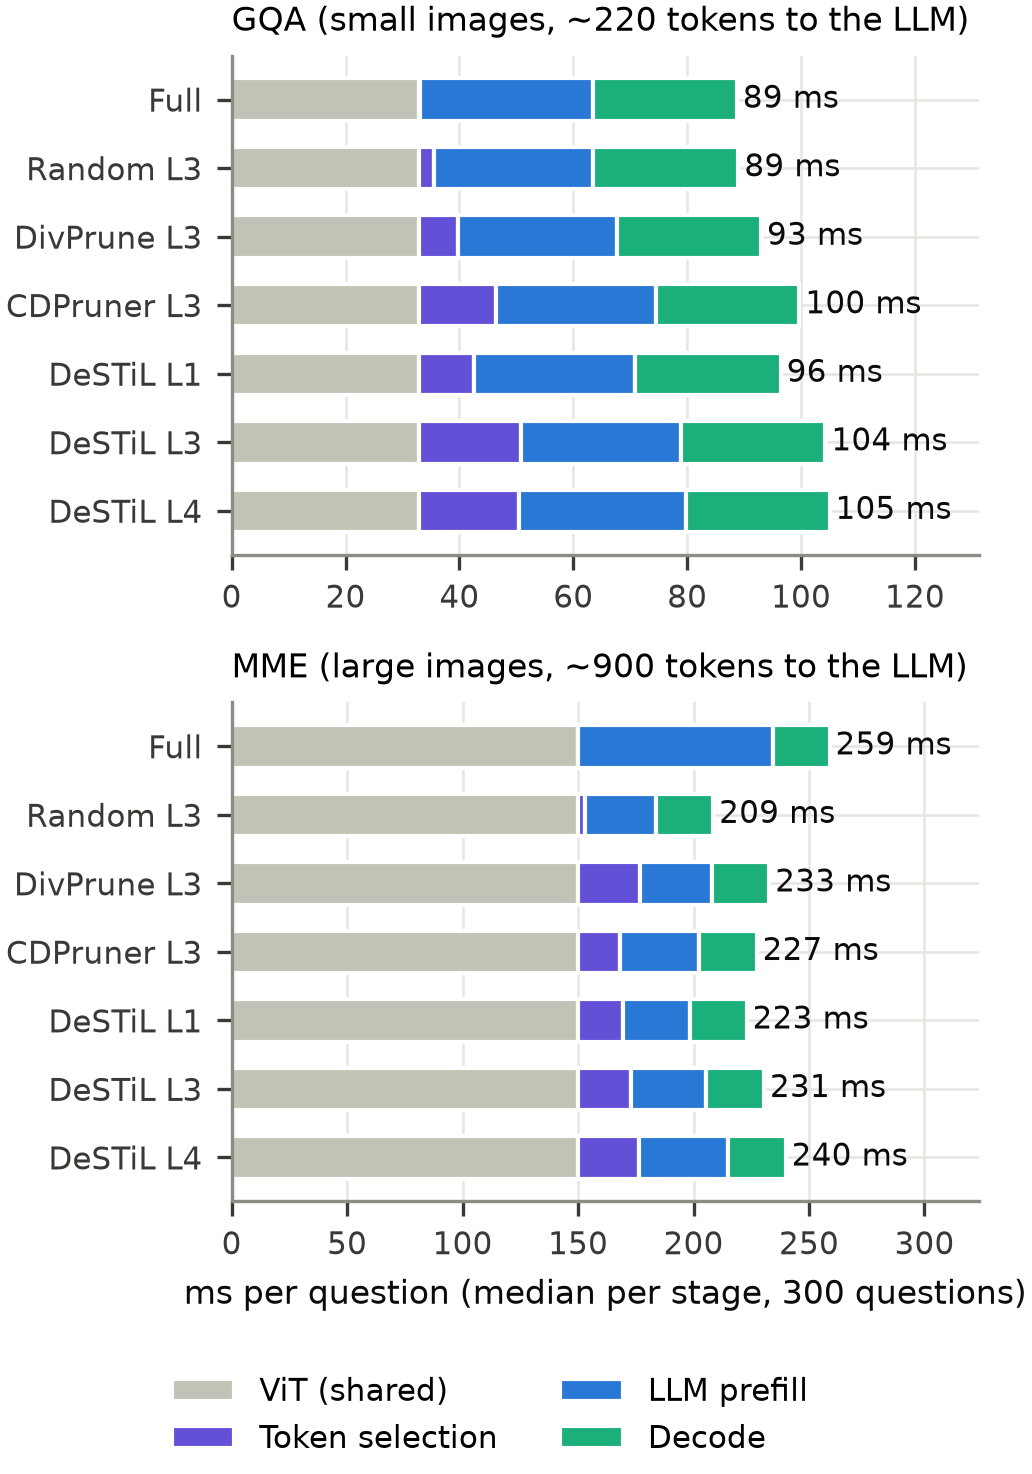
\includegraphics[width=\columnwidth]{fig_timing.png}
\caption{Qwen3-VL-2B: thời gian mỗi câu, trung vị của từng bước (ViT, chọn token, prefill, decode). FastV-style không có trong hình vì lượt chạy thêm 2 lớp LLM của nó không nằm trong phần được đo.}
\label{fig:timing}
\end{figure}

\FloatBarrier
\bibliographystyle{IEEEtran}
\bibliography{refs}

\end{document}
